\chapter{解的敏感性}
\label{chap:ode-sensitivity}

培养液里细菌的相对密度满足$\dot{x}=x(1-x)$。若初始密度测得$x(0)=1/4$，解是
\[
 x(t)=\frac{x_0\mathrm{e}^{t}}{1-x_0+x_0\mathrm{e}^{t}},\qquad x_0=\frac14,
\]
在$t=\ln3$时$x=1/2$。可是初始密度带有测量误差，增长率也只是估计值。把$x_0$改成$0.26$，$t=\ln3$时的值会差多少？把增长率改$20\%$呢？第~\ref{chap:ode-existence-continuation}章保证了解存在且唯一，却没有回答这些问题。

大多数方程写不出解的公式，因此我们要在不解方程的情况下回答它们。回答有三种精度。最粗的是整段曲线的差不超过多少，这只需要估计，由Gronwall不等式完成。其次是一阶响应：初值或参数沿某方向变一点，解沿哪个方向变、变多少，这要先证明解可微，再解一个线性方程。最后，若关心的只是由解算出的一个目标值，而参数很多，就用一次反向求解得到全部偏导数。

本章按这三种精度展开。Gronwall估计给出曲线距离的上界，并依次用于初值、参数和输入的改变。变分方程给出一阶响应。把初始状态到后续状态的关系看成映射，就得到流映射，它的Jacobian矩阵回答小区域的拉伸和体积变化，Hamilton流是其中保持体积的一类。最后由变分方程导出伴随方程。全章只讨论有限时间区间上的结论，上面的方程$\dot{x}=x(1-x)$会反复用作手算的例子。

\section{Gronwall估计}
\label{sec:odesens-gronwall}

没有解的公式，怎样比较两条解曲线？回到积分形式。解是右端的累积，两条解的差也就是右端之差的累积，而右端之差又可以由解的差控制。这样得到一个把未知量放在两边的不等式，Gronwall不等式负责把它解开。

\paragraph{两条积分方程相减}
设$\bm{x}$和$\bm{y}$在$[t_0,T]$上绝对连续，分别满足
\[
 \dot{\bm{x}}=\bm{f}(t,\bm{x}),\qquad
 \dot{\bm{y}}=\bm{f}(t,\bm{y})+\bm{r}(t),
\]
初值为$\bm{x}(t_0)=\bm{x}_0$，$\bm{y}(t_0)=\bm{y}_0$，方程几乎处处成立。这里$\bm{r}(t)$是第二条曲线相对于方程的\term{残差}（residual），表示每一时刻额外多出来的变化率。写成积分形式，
\[
 \begin{aligned}
 \bm{x}(t)&=\bm{x}_0+\int_{t_0}^{t}\bm{f}(s,\bm{x}(s))\,\mathrm{d}s,\\
 \bm{y}(t)&=\bm{y}_0+\int_{t_0}^{t}\bigl[\bm{f}(s,\bm{y}(s))+\bm{r}(s)\bigr]\,\mathrm{d}s.
 \end{aligned}
\]
记$\bm{e}(t)=\bm{y}(t)-\bm{x}(t)$，$\bm{e}_0=\bm{y}_0-\bm{x}_0$。两式相减，得到
\[
 \bm{e}(t)=\bm{e}_0+\int_{t_0}^{t}\bigl[\bm{f}(s,\bm{y}(s))-\bm{f}(s,\bm{x}(s))\bigr]\,\mathrm{d}s+\int_{t_0}^{t}\bm{r}(s)\,\mathrm{d}s.
\]

现在设右端关于状态满足Lipschitz条件，在时刻$s$的常数为$L(s)$，也就是
\[
 \lVert\bm{f}(s,\bm{y}(s))-\bm{f}(s,\bm{x}(s))\rVert_2\leq L(s)\lVert\bm{e}(s)\rVert_2.
\]
取范数并用三角不等式，$u(t)=\lVert\bm{e}(t)\rVert_2$满足
\begin{equation}
 u(t)\leq\lVert\bm{e}_0\rVert_2+\int_{t_0}^{t}\bigl[L(s)u(s)+\lVert\bm{r}(s)\rVert_2\bigr]\,\mathrm{d}s.
 \label{eq:odesens-error-inequality}
\end{equation}
式~\eqref{eq:odesens-error-inequality}两边都有$u$，并没有给出$u$的上界：要知道今天的误差，得先知道过去的误差。

\paragraph{复利的图景}
把$u$看成账户余额，$L(s)$是时刻$s$的利率，$\lVert\bm{r}(s)\rVert_2$是时刻$s$的存款速度，$\lVert\bm{e}_0\rVert_2$是本金。一小段时间$h$内，余额至多变成
\[
 u(s+h)\lesssim\bigl(1+L(s)h\bigr)u(s)+\lVert\bm{r}(s)\rVert_2h.
\]
这正是复利的递推。复利的结果可以直接写出：本金从$t_0$起计息，到$t$时乘以$\exp\int_{t_0}^{t}L$；时刻$s$存入的一小笔钱只从$s$起计息，到$t$时乘以$\exp\int_{s}^{t}L$。

图~\ref{fig:odesens-gronwall-deposits}画出了这两种钱的去向。类比也有限度：账户的利率真实发生，而式~\eqref{eq:odesens-error-inequality}只说误差“至多”按这个利率增长，真实的误差可能增长得慢，甚至缩小。Gronwall不等式给出的因此只是上界。

\begin{BookInlineFigure}
  \centering
  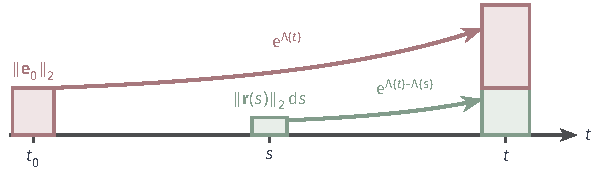
\includegraphics[width=101.9mm]{figures/06-differential-equations/01-ordinary-differential-equations/tikz/odesens-gronwall-deposits/figure.pdf}
  \caption{误差的复利账本示意。红色是初值误差$\lVert\bm{e}_0\rVert_2$，从$t_0$起一直被放大；绿色是时刻$s$处残差新注入的一小笔$\lVert\bm{r}(s)\rVert_2\,\mathrm{d}s$，只经历$s$之后的放大。时刻$t$的总上界是所有这些量放大后的和。}
  \label{fig:odesens-gronwall-deposits}
\end{BookInlineFigure}

\paragraph{Gronwall不等式}
复利的结论对一切满足该积分不等式的函数都成立，这就是\term{Gronwall不等式}（Gronwall inequality）。为了同时适用于可测输入，放大系数只要求可积。

\begin{lemma}[Gronwall不等式]
\label{lem:odesens-gronwall}
设$u:[t_0,T]\to[0,\infty)$连续，$a\geq0$是常数，$\beta,b:[t_0,T]\to[0,\infty)$可积，且对每个$t\in[t_0,T]$，
\begin{equation}
 u(t)\leq a+\int_{t_0}^{t}\bigl[\beta(s)u(s)+b(s)\bigr]\,\mathrm{d}s.
 \label{eq:odesens-gronwall-hypothesis}
\end{equation}
记$\Lambda(t)=\int_{t_0}^{t}\beta(s)\,\mathrm{d}s$。则对每个$t\in[t_0,T]$，
\begin{equation}
 u(t)\leq a\,\mathrm{e}^{\Lambda(t)}+\int_{t_0}^{t}\mathrm{e}^{\Lambda(t)-\Lambda(s)}b(s)\,\mathrm{d}s.
 \label{eq:odesens-gronwall-conclusion}
\end{equation}
\end{lemma}

\begin{proof}
记式~\eqref{eq:odesens-gronwall-hypothesis}的右端为$w(t)$。$\beta u+b$可积，所以$w$绝对连续，且几乎处处有
\[
 \dot{w}=\beta u+b.
\]
因为$\beta\geq0$，把$u\leq w$代入，得到
\[
 \dot{w}\leq\beta w+b.
\]

这是一阶线性不等式，用积分因子$\mathrm{e}^{-\Lambda}$处理。$\Lambda$绝对连续，两个绝对连续函数的乘积也绝对连续，于是几乎处处有
\[
 \frac{\mathrm{d}}{\mathrm{d}t}\bigl(\mathrm{e}^{-\Lambda}w\bigr)=\mathrm{e}^{-\Lambda}(\dot{w}-\beta w)\leq\mathrm{e}^{-\Lambda}b.
\]

从$t_0$到$t$积分，并用$w(t_0)=a$、$\Lambda(t_0)=0$，得到
\[
 \mathrm{e}^{-\Lambda(t)}w(t)\leq a+\int_{t_0}^{t}\mathrm{e}^{-\Lambda(s)}b(s)\,\mathrm{d}s.
\]
两边乘以$\mathrm{e}^{\Lambda(t)}$，再用$u\leq w$，就是式~\eqref{eq:odesens-gronwall-conclusion}。
\end{proof}

证明里$\beta\geq0$只用了一次，却不能省：把$u$放大成$w$再乘以$\beta$，不等号的方向要靠$\beta$非负。取$\beta\equiv-1$、$a=1$、$b=0$，定义
\[
 u(t)=\min\bigl\{\max\{t-1,0\},\,1/4\bigr\},\qquad t\in[0,3].
\]
它不超过$1/4$，积分$\int_0^3u$等于$15/32$，所以$1-\int_0^tu\geq17/32\geq u(t)$，假设式成立。若结论式仍成立，应有$u(3)\leq\mathrm{e}^{-3}\approx0.05$，而实际$u(3)=1/4$。负的放大率要换用微分形式处理，第~\ref{sec:odesens-initial}节会回到这一点。

\paragraph{基本误差估计}
把引理用于式~\eqref{eq:odesens-error-inequality}，就得到本章反复使用的比较定理。定理只要求两条曲线所经过的集合上有Lipschitz常数，这个集合怎样选取留给下一节。

\begin{theorem}[基本误差估计]
\label{thm:odesens-basic-estimate}
设$\bm{K}\subseteq\mathbb{R}^{n}$，曲线$\bm{x},\bm{y}:[t_0,T]\to\bm{K}$绝对连续，几乎处处满足$\dot{\bm{x}}=\bm{f}(t,\bm{x})$与$\dot{\bm{y}}=\bm{f}(t,\bm{y})+\bm{r}(t)$，其中$\bm{r}$可积。设存在可积函数$L\geq0$，使对几乎每个$t$及所有$\bm{a},\bm{b}\in\bm{K}$，
\begin{equation}
 \lVert\bm{f}(t,\bm{a})-\bm{f}(t,\bm{b})\rVert_2\leq L(t)\lVert\bm{a}-\bm{b}\rVert_2.
 \label{eq:odesens-lipschitz}
\end{equation}
记$\Lambda(t)=\int_{t_0}^{t}L(s)\,\mathrm{d}s$。则对每个$t\in[t_0,T]$，
\begin{equation}
 \lVert\bm{y}(t)-\bm{x}(t)\rVert_2\leq\mathrm{e}^{\Lambda(t)}\lVert\bm{y}_0-\bm{x}_0\rVert_2+\int_{t_0}^{t}\mathrm{e}^{\Lambda(t)-\Lambda(s)}\lVert\bm{r}(s)\rVert_2\,\mathrm{d}s.
 \label{eq:odesens-basic-estimate}
\end{equation}
\end{theorem}

\begin{proof}
由式~\eqref{eq:odesens-lipschitz}，$u=\lVert\bm{y}-\bm{x}\rVert_2$满足式~\eqref{eq:odesens-error-inequality}。在引理~\ref{lem:odesens-gronwall}中取$a=\lVert\bm{y}_0-\bm{x}_0\rVert_2$、$\beta=L$、$b=\lVert\bm{r}\rVert_2$，即得结论。
\end{proof}

常用的特殊情形是$L$为常数，且$\lVert\bm{r}(s)\rVert_2\leq\delta$。此时积分可以算出，
\begin{equation}
 \lVert\bm{y}(t)-\bm{x}(t)\rVert_2\leq\mathrm{e}^{L(t-t_0)}\lVert\bm{y}_0-\bm{x}_0\rVert_2+\delta\,\frac{\mathrm{e}^{L(t-t_0)}-1}{L}.
 \label{eq:odesens-constant-estimate}
\end{equation}

\paragraph{三个量各自怎样进入上界}
式~\eqref{eq:odesens-basic-estimate}把误差分成三个来源。初始误差进入第一项，乘以从$t_0$到$t$的全部放大。持续外力进入第二项，时刻$s$的残差只经历剩余时间的放大，所以早的残差比晚的残差放大得多。放大系数$L$只通过积分$\Lambda$进入，一段短时间内的大$L$和一段长时间内的小$L$作用相同。

图~\ref{fig:odesens-gronwall-roles}用$\dot{x}=\sin x$逐项演示，这里$\lvert\partial_x\sin x\rvert\leq1$，取$L=1$。三幅图分别只保留一个因素，蓝线是真实距离，红线是上界。

\begin{BookInlineFigure}
  \centering
  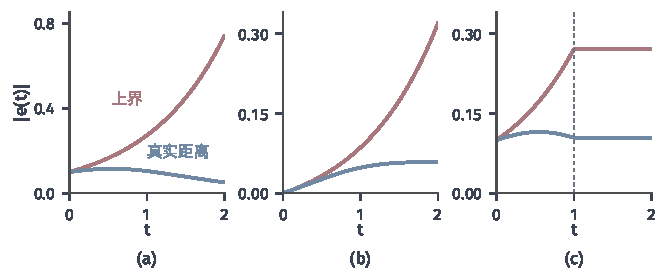
\includegraphics[width=112mm]{figures/06-differential-equations/01-ordinary-differential-equations/matplotlib/odesens-gronwall-roles/figure.pdf}
  \caption{Gronwall上界的三个成分。方程基于$\dot{x}=\sin x$，$x(0)=1$，蓝线是由数值积分得到的真实距离，红线是式~\eqref{eq:odesens-basic-estimate}的上界。(a)只有初值差$0.1$，上界$0.1\mathrm{e}^{t}$。(b)只有持续外力$r\equiv0.05$，上界$0.05(\mathrm{e}^{t}-1)$。(c)右端乘以$\beta(t)$，$\beta$在$[0,1)$上为$1$、此后为$0$，上界在$t=1$（虚线）后不再增长。}
  \label{fig:odesens-gronwall-roles}
\end{BookInlineFigure}

上界并非总是宽松的。取$\dot{x}=x$和$\dot{y}=y+0.05$，初值差$0.1$，误差方程$\dot{e}=e+0.05$可以直接解出，
\[
 e(t)=0.1\,\mathrm{e}^{t}+0.05\,(\mathrm{e}^{t}-1).
\]
这恰好是式~\eqref{eq:odesens-constant-estimate}取$L=1$、$\delta=0.05$的右端，在$t=1$时等于$0.2718+0.0859=0.3577$。可见不增加其他结构时，这个上界不能再改进。

\paragraph{去掉Lipschitz条件会怎样}
定理的结论蕴含唯一性：取$\bm{r}=\bm{0}$、$\bm{y}_0=\bm{x}_0$，上界为零。方程$\dot{x}=2\sqrt{\lvert x\rvert}$从$x(0)=0$出发有一族解，对任意$c\geq0$，
\[
 x_c(t)=\begin{cases}0,&t\leq c,\\(t-c)^2,&t>c,\end{cases}
\]
都满足方程，见图~\ref{fig:odesens-nonlipschitz-split}。比较$x_0(t)=t^2$与零解，差商是
\[
 \frac{\lvert f(t^2)-f(0)\rvert}{t^2}=\frac{2}{t},
\]
它在$t=0$附近不可积。放大系数的积分发散，式~\eqref{eq:odesens-basic-estimate}无从写起，这就是Lipschitz条件失效的具体样子。

\begin{BookInlineFigure}
  \centering
  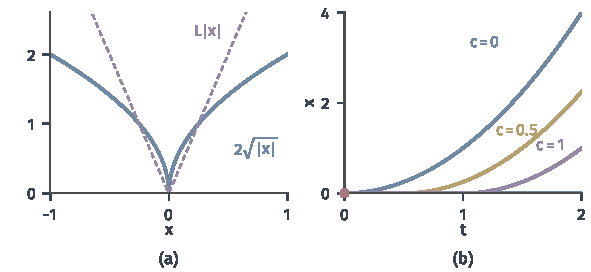
\includegraphics[width=100mm]{figures/06-differential-equations/01-ordinary-differential-equations/matplotlib/odesens-nonlipschitz-split/figure.pdf}
  \caption{没有Lipschitz条件时比较定理失效。(a)右端$2\sqrt{\lvert x\rvert}$在$x=0$处切线竖直，任何过原点的直线$L\lvert x\rvert$（紫色虚线）都压不住它。(b)同一红色初值$x(0)=0$出发的解$x_c$，$c=0,0.5,1$，蓝色水平线是零解。初值差为零，解的差却不为零。}
  \label{fig:odesens-nonlipschitz-split}
\end{BookInlineFigure}

\section{初值依赖}
\label{sec:odesens-initial}

定理~\ref{thm:odesens-basic-estimate}假设两条曲线都在$[t_0,T]$上存在，并且都留在同一个有Lipschitz常数的集合里。这对邻近初值的解并非自动成立。考虑$\dot{x}=x^2$，解是
\[
 x(t)=\frac{x_0}{1-x_0t},
\]
正初值的解在$t=1/x_0$爆炸。从$x_0=0.5$出发的解在$[0,1]$上存在，从$x_0=1.25$出发的解到$t=0.8$就没有了。

我们要回答的是：给定一条在紧区间$[t_0,T]$上存在的解，多近的初值能保证解也活到$T$，并且曲线距离可控？

\paragraph{在解的周围取一段管道}
思路是沿着已知解围一条半径为$\rho$的管道。管道是紧集，右端在里面有统一的Lipschitz常数。邻近的解只要还在管道里，Gronwall上界就成立；上界又说明它离中心线不超过$\rho/2$，碰不到管壁。图~\ref{fig:odesens-tube-continuation}中的红色虚线是一条假想的解，它要到达管壁，必须先穿过$\rho/2$的范围，这与上界矛盾。于是解出不去，也就活到了$T$。

\begin{BookInlineFigure}
  \centering
  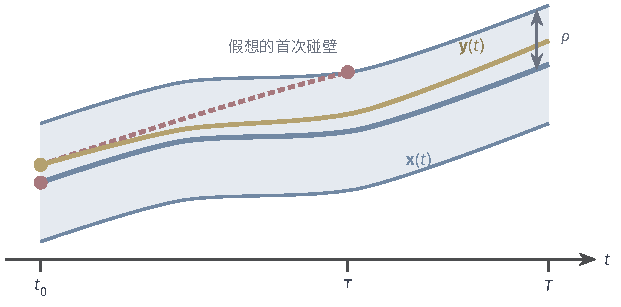
\includegraphics[width=105.2mm]{figures/06-differential-equations/01-ordinary-differential-equations/tikz/odesens-tube-continuation/figure.pdf}
  \caption{管道论证示意。浅蓝带是参考解$\bm{x}(t)$（蓝）周围半径$\rho$的管道，右端在其中有统一的Lipschitz常数。初值足够近的解$\bm{y}(t)$（黄）留在管道内。红色虚线表示假想的情形：解在$\tau$时首次碰壁，这与上界矛盾。}
  \label{fig:odesens-tube-continuation}
\end{BookInlineFigure}

图~\ref{fig:odesens-common-interval}的浅蓝带就是$\dot{x}=x^2$的管道。

\begin{BookInlineFigure}
  \centering
  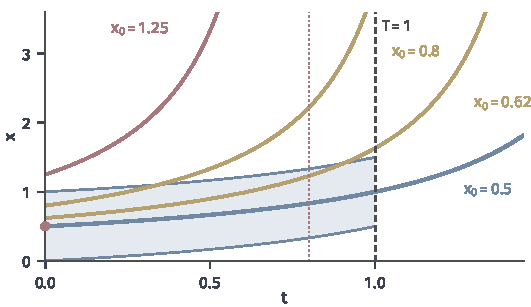
\includegraphics[width=90mm]{figures/06-differential-equations/01-ordinary-differential-equations/matplotlib/odesens-common-interval/figure.pdf}
  \caption{$\dot{x}=x^2$的邻近解。蓝色粗线从红点$x_0=0.5$出发，在$[0,1]$上存在，浅蓝带是半径$\rho=0.5$的管道。黄线$x_0=0.62$、$x_0=0.8$在$T=1$之前穿出管道，但解仍能活到$T=1$。红线$x_0=1.25$在红色点线$t=0.8$处爆炸，到不了$T=1$（灰色虚线）。}
  \label{fig:odesens-common-interval}
\end{BookInlineFigure}

证明要用第~\ref{chap:ode-existence-continuation}章的延拓结论：在局部唯一条件下，最大解若不能继续延拓，就会离开定义域内的任意紧集。也就是说，一段解如果始终留在定义域内的某个紧集里，就可以向后延伸。

\begin{theorem}[初值的局部Lipschitz依赖]
\label{thm:odesens-local-lipschitz}
设$\bm{D}\subseteq\mathbb{R}\times\mathbb{R}^{n}$是开集，$\bm{f}:\bm{D}\to\mathbb{R}^{n}$连续，且在每一点附近关于状态Lipschitz。设$\bm{x}:[t_0,T]\to\mathbb{R}^{n}$是一条解，其图像落在$\bm{D}$内。则存在$\rho>0$，使管道
\begin{equation}
 \bm{K}_\rho=\bigl\{(t,\bm{z}):t\in[t_0,T],\ \lVert\bm{z}-\bm{x}(t)\rVert_2\leq\rho\bigr\}
 \label{eq:odesens-tube}
\end{equation}
是$\bm{D}$的紧子集，$\bm{f}$在其上关于状态有统一的Lipschitz常数$L$。进一步，令$\delta=\tfrac12\rho\,\mathrm{e}^{-L(T-t_0)}$，则对每个满足$\lVert\bm{y}_0-\bm{x}_0\rVert_2\leq\delta$的$\bm{y}_0$，从$(t_0,\bm{y}_0)$出发的解在$[t_0,T]$上存在，且留在$\bm{K}_\rho$内。对两个这样的初值$\bm{y}_0$、$\bm{w}_0$，相应的解满足
\begin{equation}
 \lVert\bm{y}(t)-\bm{w}(t)\rVert_2\leq\mathrm{e}^{L(t-t_0)}\lVert\bm{y}_0-\bm{w}_0\rVert_2,\qquad t\in[t_0,T].
 \label{eq:odesens-local-lipschitz}
\end{equation}
\end{theorem}

\begin{proof}
先取管道。$\bm{x}$的图像是开集$\bm{D}$中的紧集，到$\bm{D}$的补集有正距离（$\bm{D}$是全空间时距离视为无穷）。取$\rho$小于这个距离的一半，则$\bm{K}_\rho\subset\bm{D}$，且$\bm{K}_\rho$是有界闭集，因而紧。

再说明Lipschitz常数统一。假设不然，对每个$k$有$(t_k,\bm{a}_k),(t_k,\bm{b}_k)\in\bm{K}_\rho$，使
\[
 \lVert\bm{f}(t_k,\bm{a}_k)-\bm{f}(t_k,\bm{b}_k)\rVert_2>k\lVert\bm{a}_k-\bm{b}_k\rVert_2.
\]
连续函数$\bm{f}$在紧集上有界，设界为$M$，于是$\lVert\bm{a}_k-\bm{b}_k\rVert_2<2M/k\to0$。取子列使两组点收敛到同一点$(t_\ast,\bm{z}_\ast)\in\bm{K}_\rho$。该点附近$\bm{f}$关于状态有Lipschitz常数，而$k\to\infty$与之矛盾。

现在设$\lVert\bm{y}_0-\bm{x}_0\rVert_2\leq\delta$，$\bm{y}$是最大解。令$\tau$为使$\bm{y}$在$[t_0,s]$上存在并留在$\bm{K}_\rho$内的$s\leq T$的上确界，初值在管道内部，所以$\tau>t_0$。在$[t_0,\tau)$上用定理~\ref{thm:odesens-basic-estimate}，$\bm{r}=\bm{0}$，得到
\[
 \lVert\bm{y}(t)-\bm{x}(t)\rVert_2\leq\mathrm{e}^{L(t-t_0)}\delta\leq\frac{\rho}{2}.
\]

这段解留在紧集$\bm{K}_\rho$内，由延拓结论，它可以延拓到$\tau$，且若$\tau<T$还能继续延拓到$\tau$之后。上面的不等式到$\tau$处仍成立，$\bm{y}(\tau)$离中心线不超过$\rho/2$，延拓后的一小段仍在管道内，与$\tau$的定义矛盾。所以$\tau=T$，解在闭区间$[t_0,T]$上存在且在管道内。

最后，两条解$\bm{y}$、$\bm{w}$都在$\bm{K}_\rho$内，再用一次定理~\ref{thm:odesens-basic-estimate}，就得到式~\eqref{eq:odesens-local-lipschitz}。
\end{proof}

定理中的量词值得留意。$\rho$、$L$、$\delta$都依赖给定的解和$T$，结论只在这条解附近成立，即使$\bm{f}$全局光滑也是如此。$T$越靠近这条解的爆炸时刻，管道内的$L$越大，$\delta$越小。

\begin{example}[管道的具体数字]
\label{ex:odesens-tube}
对$\dot{x}=x^2$，$x_0=1/2$，$T=1$，解$x(t)=1/(2-t)$取值在$[1/2,1]$内。取$\rho=1/2$，管道内状态在$[0,3/2]$中，$\lvert\partial_xf\rvert=2\lvert x\rvert\leq3$，所以取$L=3$。定理给出
\[
 \delta=\frac12\cdot\frac12\,\mathrm{e}^{-3}\approx0.0124.
\]

取$y_0=0.51$，它满足条件。上界给出
\[
 \lvert y(1)-x(1)\rvert\leq0.01\,\mathrm{e}^{3}\approx0.201.
\]
真实值可以直接算，
\[
 y(1)-x(1)=\frac{0.51}{0.49}-1\approx0.0408.
\]
上界偏大约五倍，因为它用整条管道上最坏的$L$。$\delta$也偏保守：实际上任何$y_0<1$的解都能活到$T=1$。定理的作用是不解方程也给出保证。
\end{example}

\paragraph{连续依赖与Lipschitz依赖}
定理~\ref{thm:odesens-local-lipschitz}的结论是\term{Lipschitz依赖}（Lipschitz dependence）：解的差不超过初值差的常数倍。更弱的要求是\term{连续依赖}（continuous dependence）：对任意$\varepsilon>0$，存在$\delta>0$，初值差小于$\delta$时，$[t_0,T]$上的解差小于$\varepsilon$。两者在依赖的“速度”上不同，所需条件也不同，见表~\ref{tab:odesens-dependence}。

\begin{BookInlineTable}
  \centering
  \caption{初值依赖的层次。结论都是给定解附近、紧时间段上的局部结论。}
  \label{tab:odesens-dependence}
  \begin{tabular}{p{28mm}p{32mm}p{38mm}}
    \toprule
    右端条件 & 依赖性质 & 例子 \\
    \midrule
    连续，解不唯一 & 流映射没有定义 & $\dot{x}=2\sqrt{\lvert x\rvert}$ \\
    连续，解唯一 & 连续依赖 & $\dot{x}=-x\ln\lvert x\rvert$ \\
    局部Lipschitz & Lipschitz依赖 & $\dot{x}=\lvert x\rvert$ \\
    连续可微 & 可微依赖（第~\ref{sec:odesens-variational}节） & $\dot{x}=x(1-x)$ \\
    \bottomrule
  \end{tabular}
\end{BookInlineTable}

第二行的结论是：右端仅连续时，只要过每个邻近初值的解都唯一，连续依赖仍然成立。证明需要用到等度连续曲线族的紧性（Arzelà--Ascoli定理）并配合延拓，篇幅较长，读者可查阅常微分方程教材。其机制是：邻近初值的解构成一族等度连续的曲线，任何收敛子列的极限都是初值问题的解，唯一性迫使极限只能是原来那条解。这个论证没有给出收敛的速度。

没有速度保证的情形确实存在。方程$\dot{x}=-x\ln\lvert x\rvert$（约定在$x=0$处右端为$0$）在$x=0$处斜率趋于无穷，右端不Lipschitz，但解仍唯一。对$0<x_0<1$，令$v=\ln x$，方程化为$\dot{v}=-v$，于是
\[
 x(t)=x_0^{\mathrm{e}^{-t}}.
\]
若有解从$0$离开，变量$v$要在有限时间内从$-\infty$变为有限值，而$\dot{v}=-v$的解不会在有限时间内从无穷回来，所以$x\equiv0$是从$0$出发的唯一解。

取$t=\ln2$，解的映射是$x_0\mapsto\sqrt{x_0}$。$x_0=10^{-4}$时解是$10^{-2}$，初值差被放大$100$倍；$x_0=10^{-8}$时放大$10^{4}$倍。比值$\sqrt{x_0}/x_0$没有上界，所以不存在Lipschitz常数。依赖仍然连续，因为$x_0\to0$时$\sqrt{x_0}\to0$，见图~\ref{fig:odesens-holder-flow}。

\begin{BookInlineFigure}
  \centering
  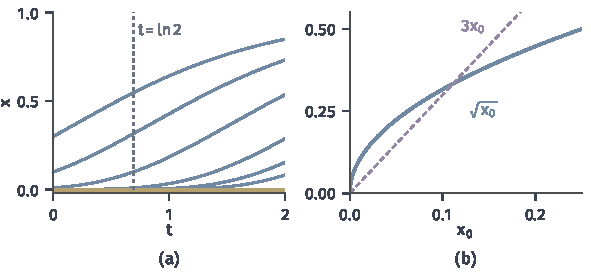
\includegraphics[width=100mm]{figures/06-differential-equations/01-ordinary-differential-equations/matplotlib/odesens-holder-flow/figure.pdf}
  \caption{连续依赖但不Lipschitz。(a)$\dot{x}=-x\ln x$从$x_0=10^{-8},10^{-6},10^{-4},10^{-2},0.1,0.3$出发的解（蓝）和零解（黄）。极小的初值很快被拉开。(b)$t=\ln2$时的解映射$\sqrt{x_0}$，在$x_0=0$处切线竖直，任何直线（紫色虚线）在原点附近都压不住它。}
  \label{fig:odesens-holder-flow}
\end{BookInlineFigure}

\paragraph{有限时间上界不是长期稳定判据}
式~\eqref{eq:odesens-local-lipschitz}的常数$\mathrm{e}^{L(T-t_0)}$随$T$指数增长。它只是有限时间的上界，不能用来判断解在长时间下靠拢还是分离。图~\ref{fig:odesens-bound-vs-true}用$L=1$的三个方程作对比，初值差都是$0.01$。

\begin{BookInlineFigure}
  \centering
  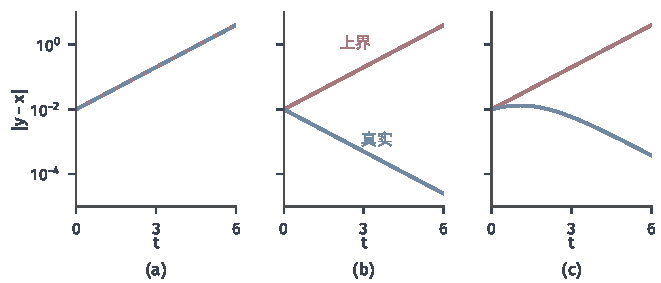
\includegraphics[width=112mm]{figures/06-differential-equations/01-ordinary-differential-equations/matplotlib/odesens-bound-vs-true/figure.pdf}
  \caption{同一个上界$0.01\,\mathrm{e}^{t}$（红）与三种真实距离（蓝，对数纵轴）。(a)$\dot{x}=x$，上界就是真实距离。(b)$\dot{x}=-x$，真实距离按$\mathrm{e}^{-t}$衰减。(c)$\dot{x}=x(1-x)$，$x_0=0.25$，距离先增后减。}
  \label{fig:odesens-bound-vs-true}
\end{BookInlineFigure}

三种情形的$L$相同，长期行为却完全不同，因为$L$只记录了$\lvert\partial_xf\rvert$的大小，丢掉了符号。反过来，$\mathrm{e}^{L(T-t_0)}$在任何固定的$T$上都有限，这也不说明解在$T\to\infty$时保持靠近。长期行为需要吸引性、不变集等额外结构，可参考\BookChapterRef{chap:dynamical-systems-long-term}{卷九第1章“动力系统与轨迹的长期行为”}。

\paragraph{保留符号信息}
能否在估计里留下符号？引理~\ref{lem:odesens-gronwall}的积分形式要求$\beta\geq0$，但如果直接对距离的平方求导，放大率可以取负。为此把Lipschitz条件换成只约束相互靠近方向的条件，称为\term{单侧Lipschitz条件}（one-sided Lipschitz condition）。

\begin{lemma}[单侧Lipschitz估计]
\label{lem:odesens-one-sided}
设$\bm{x},\bm{y}:[t_0,T]\to\bm{K}$绝对连续，几乎处处满足$\dot{\bm{x}}=\bm{f}(t,\bm{x})$、$\dot{\bm{y}}=\bm{f}(t,\bm{y})$。设实值函数$\mu$可积（可以取负值），且对几乎每个$t$及所有$\bm{a},\bm{b}\in\bm{K}$，
\begin{equation}
 \bigl\langle\bm{f}(t,\bm{a})-\bm{f}(t,\bm{b}),\,\bm{a}-\bm{b}\bigr\rangle\leq\mu(t)\lVert\bm{a}-\bm{b}\rVert_2^2.
 \label{eq:odesens-one-sided}
\end{equation}
则对每个$t\in[t_0,T]$，
\begin{equation}
 \lVert\bm{y}(t)-\bm{x}(t)\rVert_2\leq\lVert\bm{y}_0-\bm{x}_0\rVert_2\,\exp\int_{t_0}^{t}\mu(s)\,\mathrm{d}s.
 \label{eq:odesens-one-sided-bound}
\end{equation}
\end{lemma}

\begin{proof}
令$v=\lVert\bm{y}-\bm{x}\rVert_2^2$，$v$绝对连续。由式~\eqref{eq:odesens-one-sided}，几乎处处有
\[
 \dot{v}=2\bigl\langle\bm{f}(t,\bm{y})-\bm{f}(t,\bm{x}),\,\bm{y}-\bm{x}\bigr\rangle\leq2\mu v.
\]
记$M(t)=\int_{t_0}^{t}\mu$，乘以积分因子后得到
\[
 \frac{\mathrm{d}}{\mathrm{d}t}\bigl(\mathrm{e}^{-2M}v\bigr)\leq0.
\]
所以$v(t)\leq\mathrm{e}^{2M(t)}v(t_0)$，开方即得结论。
\end{proof}

对$\dot{x}=-x$，条件式成立且$\mu=-1$，式~\eqref{eq:odesens-one-sided-bound}恰好是真实的$\mathrm{e}^{-t}$衰减。对$\dot{x}=-x^3$，
\[
 (a-b)(-a^3+b^3)=-(a-b)^2(a^2+ab+b^2)\leq0,
\]
可取$\mu=0$，而这个右端在$\mathbb{R}$上没有全局Lipschitz常数。这样的方程上任意两条解的距离不增，这比用$L$的上界强得多。该结论同样只陈述了给定时间段上的比较，并不涉及平衡点的吸引。

\section{参数与输入扰动}
\label{sec:odesens-parameter-input}

初值只是数据的一部分。方程里的系数是估计出来的，外部输入有噪声，方程本身也只是对真实规律的近似。这些改变看上去性质各异，其实都改变了同一件事：曲线每一时刻的变化率。它们都可以写成积分方程中的残差，于是定理~\ref{thm:odesens-basic-estimate}一次解决全部情形。

\paragraph{统一成积分方程中的扰动}
设$\bm{x}$解$\dot{\bm{x}}=\bm{f}(t,\bm{x})$，$\bm{y}$解被改变的方程$\dot{\bm{y}}=\tilde{\bm{f}}(t,\bm{y})$。把$\bm{y}$的方程改写成
\[
 \dot{\bm{y}}=\bm{f}(t,\bm{y})+\bm{r}(t),\qquad
 \bm{r}(t)=\tilde{\bm{f}}(t,\bm{y}(t))-\bm{f}(t,\bm{y}(t)).
\]
这里$\bm{r}$沿着曲线$\bm{y}$取值，是一个只依赖时间的函数。图~\ref{fig:odesens-perturbation-sources}列出了各种改变的去向。

\begin{BookInlineFigure}
  \centering
  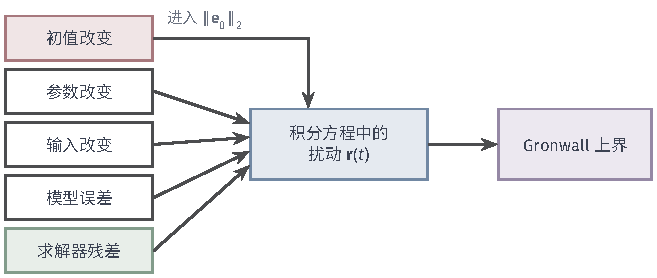
\includegraphics[width=111.2mm]{figures/06-differential-equations/01-ordinary-differential-equations/tikz/odesens-perturbation-sources/figure.pdf}
  \caption{各类改变进入同一个估计的路径。初值改变进入起点的差，参数、输入、模型与数值计算的改变都写成随时间变化的残差$\bm{r}(t)$，再由式~\eqref{eq:odesens-basic-estimate}转成曲线距离的上界。}
  \label{fig:odesens-perturbation-sources}
\end{BookInlineFigure}

\begin{theorem}[右端扰动下的比较]
\label{thm:odesens-perturbation}
设$\bm{x},\bm{y}:[t_0,T]\to\bm{K}$绝对连续，分别几乎处处满足$\dot{\bm{x}}=\bm{f}(t,\bm{x})$、$\dot{\bm{y}}=\tilde{\bm{f}}(t,\bm{y})$。设$\bm{f}$在$\bm{K}$上满足式~\eqref{eq:odesens-lipschitz}，$L$可积，且残差
\begin{equation}
 \varepsilon(t)=\bigl\lVert\tilde{\bm{f}}(t,\bm{y}(t))-\bm{f}(t,\bm{y}(t))\bigr\rVert_2
 \label{eq:odesens-residual}
\end{equation}
可积。记$\Lambda(t)=\int_{t_0}^{t}L$。则
\begin{equation}
 \lVert\bm{y}(t)-\bm{x}(t)\rVert_2\leq\mathrm{e}^{\Lambda(t)}\lVert\bm{y}_0-\bm{x}_0\rVert_2+\int_{t_0}^{t}\mathrm{e}^{\Lambda(t)-\Lambda(s)}\varepsilon(s)\,\mathrm{d}s.
 \label{eq:odesens-perturbation-bound}
\end{equation}
\end{theorem}

\begin{proof}
取定理前定义的残差$\bm{r}$，则$\lVert\bm{r}\rVert_2=\varepsilon$，$\bm{y}$满足定理~\ref{thm:odesens-basic-estimate}中带残差的方程。代入式~\eqref{eq:odesens-basic-estimate}即得结论。
\end{proof}

定理只要求$\bm{f}$有Lipschitz常数，对$\tilde{\bm{f}}$没有要求，它甚至可以不连续。这在比较真实系统与简化模型时有用：真实规律$\tilde{\bm{f}}$往往未知也不光滑，只要它的轨迹$\bm{y}$存在，并且能估计模型在这条轨迹上的误差$\varepsilon$。定理的$\bm{y}$仍须事先知道留在$\bm{K}$内；$\bm{f}$与$\tilde{\bm{f}}$足够接近时，第~\ref{sec:odesens-initial}节的管道论证可以保证这一点。

\paragraph{参数改变}
设右端依赖参数$\bm{\theta}$，且关于参数满足
\[
 \lVert\bm{f}(t,\bm{a},\tilde{\bm{\theta}})-\bm{f}(t,\bm{a},\bm{\theta})\rVert_2\leq\ell(t)\lVert\tilde{\bm{\theta}}-\bm{\theta}\rVert_2,
\]
其中$\ell$可积。此时残差不超过$\ell(s)$乘以参数差的范数，初值相同时，式~\eqref{eq:odesens-perturbation-bound}化为
\begin{equation}
 \lVert\bm{y}(t)-\bm{x}(t)\rVert_2\leq\lVert\tilde{\bm{\theta}}-\bm{\theta}\rVert_2\int_{t_0}^{t}\mathrm{e}^{\Lambda(t)-\Lambda(s)}\ell(s)\,\mathrm{d}s.
 \label{eq:odesens-parameter-bound}
\end{equation}
所以解在紧时间段上Lipschitz依赖参数，前提与初值情形相同。

\begin{example}[增长率改变$20\%$]
\label{ex:odesens-parameter-bound}
考虑$\dot{x}=\theta x(1-x)$，$x_0=1/4$，比较$\theta=1$与$\tilde{\theta}=1.2$在$T=\ln3$时的值。解都留在$\bm{K}=[0,1]$内，$\theta=1$的右端关于$x$的导数是$1-2x$，取$L=1$。残差是
\[
 r(s)=0.2\,y(s)\bigl(1-y(s)\bigr),\qquad \lvert r(s)\rvert\leq0.05.
\]

用$\lvert r\rvert\leq0.05$的粗略界，由式~\eqref{eq:odesens-constant-estimate}得到
\[
 \lvert y(T)-x(T)\rvert\leq0.05\,(\mathrm{e}^{T}-1)=0.1.
\]
若把残差沿$y$的实际值代入式~\eqref{eq:odesens-perturbation-bound}，数值积分得到上界$0.0901$。真实差是$y(T)-x(T)=0.5547-0.5=0.0547$。
\end{example}

图~\ref{fig:odesens-parameter-bound}显示了$[0,3]$上的情况。上界在$t$较大时远离真实差，原因和图~\ref{fig:odesens-bound-vs-true}(c)相同：$L=1$对应$x$靠近$0$时的增长，而$x$靠近$1$时真实的放大率是负的。

\begin{BookInlineFigure}
  \centering
  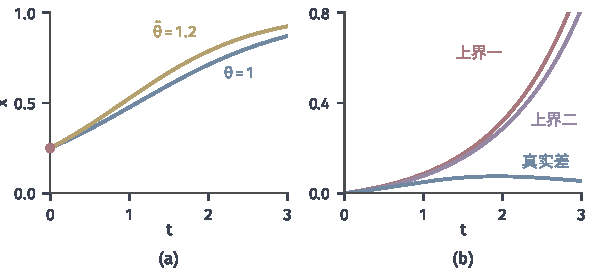
\includegraphics[width=100mm]{figures/06-differential-equations/01-ordinary-differential-equations/matplotlib/odesens-parameter-bound/figure.pdf}
  \caption{参数改变对$\dot{x}=\theta x(1-x)$的影响，$x_0=1/4$。(a)$\theta=1$（蓝）与$\tilde\theta=1.2$（黄）的解。(b)两解的真实差（蓝）、用$\lvert r\rvert\leq0.05$的上界一（红）和用残差实际值的上界二（紫）。}
  \label{fig:odesens-parameter-bound}
\end{BookInlineFigure}

\paragraph{输入改变}
设方程是$\dot{\bm{x}}=\bm{f}(t,\bm{x},\bm{g}(t))$，$\bm{g}$是可测的外部输入。应该用什么范数衡量输入的差？答案取决于右端怎样依赖输入，我们看三种情形。

设右端关于输入值Lipschitz，
\[
 \lVert\bm{f}(t,\bm{a},\tilde{\bm{g}})-\bm{f}(t,\bm{a},\bm{g})\rVert_2\leq\ell(t)\lVert\tilde{\bm{g}}-\bm{g}\rVert_2.
\]
线性输入$\bm{f}=\bm{a}(t,\bm{x})+\bm{B}(t)\bm{g}$就是这样，$\ell(t)=\lVert\bm{B}(t)\rVert_2$。此时$\varepsilon$由输入差的加权积分控制，
\begin{equation}
 \int_{t_0}^{T}\varepsilon(s)\,\mathrm{d}s\leq\int_{t_0}^{T}\ell(s)\,\lVert\tilde{\bm{g}}(s)-\bm{g}(s)\rVert_2\,\mathrm{d}s.
 \label{eq:odesens-input-l1}
\end{equation}
这里合适的度量是积分范数，也就是$L^1$范数，瞬时的巨大偏差只要持续够短，影响就小。图~\ref{fig:odesens-input-norms}(a)中方程为$\dot{x}=-x+g$，偏差是$[1,1.02)$上高度$5$的脉冲，积分等于$0.1$。解的差不超过$0.1$，实际在$t=1.02$时达到$5(1-\mathrm{e}^{-0.02})\approx0.099$，然后衰减，到$t=2$时约为$0.037$。

\begin{BookInlineFigure}
  \centering
  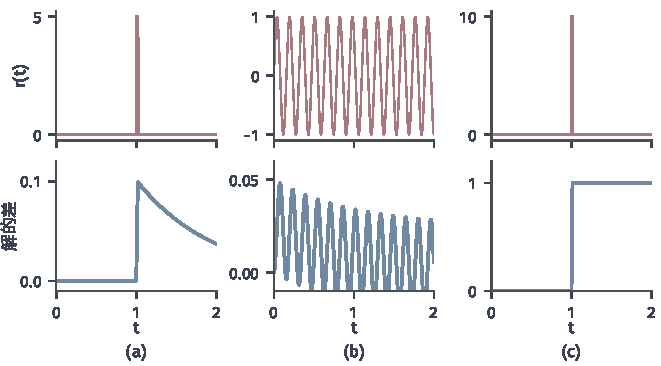
\includegraphics[width=112mm]{figures/06-differential-equations/01-ordinary-differential-equations/matplotlib/odesens-input-norms/figure.pdf}
  \caption{输入差的大小与解的差。上行是输入偏差$r(t)$，下行是解的差。(a)$\dot{x}=-x+g$，脉冲高$5$、宽$0.02$，积分$0.1$，解的差不超过$0.1$。(b)$\dot{x}=-x+g$，偏差$\sin40t$，积分范数约$1.27$，解的差却不超过$0.05$。(c)$\dot{x}=g^2$，脉冲高$10$、宽$0.01$，积分同为$0.1$，解的差却达到$1$。}
  \label{fig:odesens-input-norms}
\end{BookInlineFigure}

式~\eqref{eq:odesens-input-l1}是充分条件，不是必要条件。图~\ref{fig:odesens-input-norms}(b)的偏差$\sin40t$在$[0,2]$上的积分范数约为$1.27$，解的差却不超过$0.05$。原因是正负部分抵消，在加性输入下真正起作用的是偏差的累积$\int_{t_0}^{t}\bm{r}(s)\,\mathrm{d}s$，这里它不超过$2/40=0.05$。

非线性依赖就不同了。方程$\dot{x}=g^2$的残差是$\tilde{g}^2-g^2$，关于$g$的增长率随$\lvert g\rvert$变大。取$g\equiv0$，$\tilde{g}$是$[1,1+w)$上高度$A$的脉冲，
\[
 \int_0^2\lvert\tilde{g}-g\rvert\,\mathrm{d}t=Aw,\qquad y(2)-x(2)=A^2w.
\]
令$A=10$、$w=0.01$，输入差的积分只有$0.1$，解的差却是$1$，见图~\ref{fig:odesens-input-norms}(c)。让$A\to\infty$并保持$A^2w=1$，积分范数趋于零而解差不变。所以这里$L^1$小不足以保证解差小。

补救有两条路。若所有输入的值都限制在$\lVert\bm{g}\rVert_2\leq M$内，右端在这个范围内关于$\bm{g}$有常数$\ell=2M$，式~\eqref{eq:odesens-input-l1}恢复成立，$M$进入常数；上例$M=10$，$\ell\cdot Aw=20\times0.1=2$，确实不小于真实的$1$。另一条路是用更强的范数：一致范数$\sup_t\lVert\tilde{\bm{g}}-\bm{g}\rVert_2$小，就排除了高而窄的脉冲，只是它对孤立的短暂偏差过于敏感。

\paragraph{可测输入的条件}
上面的估计都只用到残差可积，没有用到输入的连续性。分段切换的输入、一般可测的输入都在其中，此时解是绝对连续函数，方程几乎处处成立。沿用第~\ref{chap:ode-existence-continuation}章的Carathéodory条件，右端沿解的复合是可测且局部可积的，式~\eqref{eq:odesens-residual}的$\varepsilon$因而有意义。但要得到定理~\ref{thm:odesens-basic-estimate}的结论，仍需要对时间可积的状态Lipschitz系数$L(t)$，这不是可测性能推出的。

\paragraph{方程的敏感性与求解器误差}
数值解也可以放进这个框架，这样能把两种常被混淆的误差分开。下面的计算只用定理的结构，数值方法本身放在第~\ref{chap:ode-numerical-methods}章。设网格$t_k=t_0+kh$，从$\bm{x}^{(0)}=\bm{x}_0$出发按
\[
 \bm{x}^{(k+1)}=\bm{x}^{(k)}+h\,\bm{f}(t_k,\bm{x}^{(k)})
\]
前进，把各点连成折线$\bm{y}(t)$。折线绝对连续，它的残差是$\bm{r}(s)=\dot{\bm{y}}(s)-\bm{f}(s,\bm{y}(s))$。

代入式~\eqref{eq:odesens-basic-estimate}，全局误差的上界是残差与放大因子乘积的积分。残差由求解器决定，步长越小残差越小。放大因子$\mathrm{e}^{\Lambda(t)-\Lambda(s)}$由方程决定，与求解器无关。前者是求解器的误差来源，后者是问题本身的敏感性。

\begin{example}[同一求解器，两个方程]
\label{ex:odesens-problem-solver}
取$\dot{x}=ax$，$x_0=1$，$h=1/4$，$T=1$，$a=\pm1$。在$[t_k,t_{k+1})$上，折线是$y(s)=x^{(k)}(1+a(s-t_k))$，于是
\[
 r(s)=\dot{y}-ay=-a^2x^{(k)}(s-t_k).
\]
方程线性，误差方程$\dot{e}=ae+r$可以精确求解，初值差为零时
\[
 y(1)-\mathrm{e}^{a}=\int_0^1\mathrm{e}^{a(1-s)}r(s)\,\mathrm{d}s.
\]

$a=1$时，$x^{(k)}$依次是$1,\,1.25,\,1.5625,\,1.9531,\,2.4414$；$a=-1$时依次是$1,\,0.75,\,0.5625,\,0.4219,\,0.3164$。逐段积分，得到
\[
 a=1:\ y(1)-\mathrm{e}=-0.2769,\qquad a=-1:\ y(1)-\mathrm{e}^{-1}=-0.0515.
\]
\end{example}

图~\ref{fig:odesens-problem-vs-solver}把三个量画在一起。两个方程的残差都是锯齿形，大小同为$h$的量级。权重却相反：$a=1$时早期残差被放大$\mathrm{e}^{1-s}>1$倍，$a=-1$时被缩小。误差相差五倍多，主要来自方程，而不是求解器。

\begin{BookInlineFigure}
  \centering
  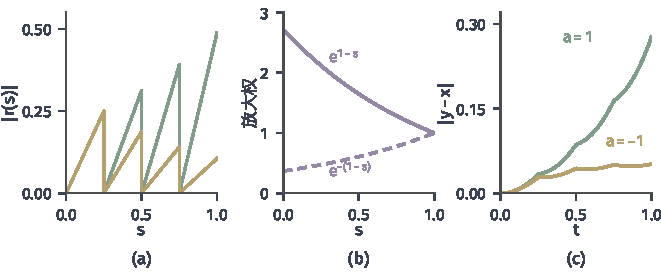
\includegraphics[width=112mm]{figures/06-differential-equations/01-ordinary-differential-equations/matplotlib/odesens-problem-vs-solver/figure.pdf}
  \caption{同一求解器在$\dot{x}=ax$上的表现，$h=1/4$，绿线$a=1$，黄线$a=-1$。(a)Euler折线的残差$\lvert r(s)\rvert$，由求解器决定。(b)放大权$\mathrm{e}^{a(1-s)}$，由方程决定（紫实线$a=1$，紫虚线$a=-1$）。(c)累积后的误差。}
  \label{fig:odesens-problem-vs-solver}
\end{BookInlineFigure}

因此，问题敏感时，再精细的求解器也只能把残差压小，放大因子还在；问题不敏感时，粗糙的残差也不至于造成大的全局误差。把解算准需要两者配合，这两者不可相互替代。


\section{变分方程}
\label{sec:odesens-variational}

Gronwall估计只回答“差多少”，不回答“往哪边差”，得到的常数也往往偏大。若解关于数据可微，初值沿某方向变一点时，解的变化就可以用一个线性方程精确算到一阶。这需要先弄清楚解什么时候可微。

\paragraph{连续依赖不能推出可微依赖}
方程$\dot{x}=\lvert x\rvert$的右端全局Lipschitz，$L=1$，解对初值Lipschitz依赖。可是$x_0>0$时解是$x_0\mathrm{e}^{t}$，$x_0<0$时解是$x_0\mathrm{e}^{-t}$，所以
\[
 \varphi_1(x_0)=\begin{cases}\mathrm{e}\,x_0,&x_0\geq0,\\x_0/\mathrm{e},&x_0<0.\end{cases}
\]
$\varphi_1$在$x_0=0$处左导数为$1/\mathrm{e}$，右导数为$\mathrm{e}$，不可微，见图~\ref{fig:odesens-kink}。Lipschitz依赖只限制了差商的大小，并不保证差商有极限。要谈导数，右端本身要可微。

\begin{BookInlineFigure}
  \centering
  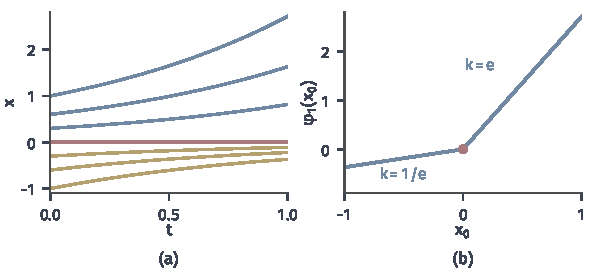
\includegraphics[width=100mm]{figures/06-differential-equations/01-ordinary-differential-equations/matplotlib/odesens-kink/figure.pdf}
  \caption{Lipschitz依赖而不可微。(a)$\dot{x}=\lvert x\rvert$的解：正初值（蓝）按$\mathrm{e}^{t}$增长，负初值（黄）按$\mathrm{e}^{-t}$衰减，红线是零解。(b)$t=1$时的解映射，在红点$x_0=0$处有折点，左右斜率分别为$1/\mathrm{e}$与$\mathrm{e}$。}
  \label{fig:odesens-kink}
\end{BookInlineFigure}

\paragraph{形式推导}
先假设可以求导，看导数应当满足什么方程。设$\bm{x}(t;\bm{x}_0,\bm{\theta})$解
\[
 \dot{\bm{x}}=\bm{f}(t,\bm{x},\bm{\theta}),\qquad \bm{x}(t_0)=\bm{x}_0,
\]
参考解记为$\bm{x}(t)$。沿方向$(\bm{v},\bm{w})$扰动，考虑$\bm{x}(t;\bm{x}_0+\varepsilon\bm{v},\bm{\theta}+\varepsilon\bm{w})$。把积分方程对$\varepsilon$在$0$处求导，记$\bm{z}(t)$为解的方向导数，由链式法则，
\[
 \bm{z}(t)=\bm{v}+\int_{t_0}^{t}\bigl[\bm{A}(s)\bm{z}(s)+\bm{B}(s)\bm{w}\bigr]\,\mathrm{d}s,
\]
其中两个系数沿参考解取值：
\begin{equation}
 \bm{A}(t)=\partial_{\bm{x}}\bm{f}\bigl(t,\bm{x}(t),\bm{\theta}\bigr),\qquad
 \bm{B}(t)=\partial_{\bm{\theta}}\bm{f}\bigl(t,\bm{x}(t),\bm{\theta}\bigr).
 \label{eq:odesens-coefficients}
\end{equation}
这就是
\begin{equation}
 \dot{\bm{z}}=\bm{A}(t)\bm{z}+\bm{B}(t)\bm{w},\qquad \bm{z}(t_0)=\bm{v},
 \label{eq:odesens-variational}
\end{equation}
称为沿参考解的\term{变分方程}（variational equation）。

原方程是非线性的，变分方程却是线性的，系数是沿已知轨迹取值的时变矩阵，第~\ref{chap:linear-differential-systems}章的工具全部可用。上面的推导把求导和积分交换了，也默认了导数存在，下面的定理补上这两点。

\begin{theorem}[解的可微依赖]
\label{thm:odesens-differentiable}
设$\bm{U}\subseteq\mathbb{R}^{n}$、$\bm{\Theta}\subseteq\mathbb{R}^{p}$是开集，取值于$\mathbb{R}^{n}$的右端$\bm{f}$定义在$[t_0,T]\times\bm{U}\times\bm{\Theta}$上，满足：对固定的$(\bm{a},\bm{\theta})$关于$t$可测；对几乎每个$t$，关于$(\bm{a},\bm{\theta})$连续可微。设$\bm{x}:[t_0,T]\to\bm{U}$是参数$\bm{\theta}$、初值$\bm{x}_0$的绝对连续解，并设存在$\rho>0$与可积函数$m\geq0$，使闭管道$\lVert\bm{a}-\bm{x}(t)\rVert_2\leq\rho$落在$\bm{U}$内，闭球$\lVert\bm{\vartheta}-\bm{\theta}\rVert_2\leq\rho$落在$\bm{\Theta}$内，且在其上对几乎每个$t$有
\begin{equation}
 \lVert\partial_{\bm{x}}\bm{f}(t,\bm{a},\bm{\vartheta})\rVert_2\leq m(t),\qquad
 \lVert\partial_{\bm{\theta}}\bm{f}(t,\bm{a},\bm{\vartheta})\rVert_2\leq m(t).
 \label{eq:odesens-derivative-bound}
\end{equation}
则存在$\delta>0$，当$\lVert\bm{v}\rVert_2+\lVert\bm{w}\rVert_2<\delta$时，初值$\bm{x}_0+\bm{v}$、参数$\bm{\theta}+\bm{w}$的解$\bm{y}$在$[t_0,T]$上存在且唯一，并且
\begin{equation}
 \sup_{t\in[t_0,T]}\bigl\lVert\bm{y}(t)-\bm{x}(t)-\bm{z}(t)\bigr\rVert_2=o\bigl(\lVert\bm{v}\rVert_2+\lVert\bm{w}\rVert_2\bigr),
 \label{eq:odesens-differentiable}
\end{equation}
其中$\bm{z}$是变分方程~\eqref{eq:odesens-variational}的解。
\end{theorem}

\begin{proof}
记扰动的大小为
\[
 \lVert\bm{\eta}\rVert=\lVert\bm{v}\rVert_2+\lVert\bm{w}\rVert_2,
\]
并记$M=\int_{t_0}^{T}m$。

\emph{第一步，解的存在与线性控制。}由式~\eqref{eq:odesens-derivative-bound}和中值不等式，右端在管道内关于状态有Lipschitz系数$m(t)$，关于参数有系数$m(t)$。按定理~\ref{thm:odesens-local-lipschitz}的管道论证，把常数$L$换成可积系数$m(t)$，并使用第~\ref{chap:ode-existence-continuation}章Carathéodory情形的延拓结论，只要$\delta$足够小，$\bm{y}$就在$[t_0,T]$上存在并留在管道内。由式~\eqref{eq:odesens-perturbation-bound}，取残差$\varepsilon\leq m\lVert\bm{w}\rVert_2$，
\[
 \lVert\bm{y}(t)-\bm{x}(t)\rVert_2\leq\mathrm{e}^{M}\lVert\bm{v}\rVert_2+M\mathrm{e}^{M}\lVert\bm{w}\rVert_2\leq C\lVert\bm{\eta}\rVert,
\]
其中$C=(1+M)\mathrm{e}^{M}$。

\emph{第二步，写出余项的方程。}记$\bm{\Delta}=\bm{y}-\bm{x}$，$\bm{R}=\bm{\Delta}-\bm{z}$，则$\bm{R}(t_0)=\bm{0}$。对几乎每个固定的$t$，沿线段$\sigma\mapsto(\bm{x}+\sigma\bm{\Delta},\bm{\theta}+\sigma\bm{w})$用微积分基本定理，
\[
 \bm{f}(t,\bm{y},\bm{\theta}+\bm{w})-\bm{f}(t,\bm{x},\bm{\theta})
 =\int_0^1\bigl[\partial_{\bm{x}}\bm{f}^{\sigma}\,\bm{\Delta}+\partial_{\bm{\theta}}\bm{f}^{\sigma}\,\bm{w}\bigr]\,\mathrm{d}\sigma,
\]
$\partial\bm{f}^{\sigma}$表示在线段上$\sigma$处取值。减去$\bm{A}\bm{z}+\bm{B}\bm{w}$，得到
\[
 \dot{\bm{R}}=\bm{A}\bm{R}+\bm{E},\qquad
 \bm{E}(t)=\int_0^1\bigl[(\partial_{\bm{x}}\bm{f}^{\sigma}-\bm{A})\bm{\Delta}+(\partial_{\bm{\theta}}\bm{f}^{\sigma}-\bm{B})\bm{w}\bigr]\,\mathrm{d}\sigma.
\]

\emph{第三步，估计$\bm{E}$。}定义
\[
 \omega_{\bm{\eta}}(t)=\sup\bigl(\lVert\partial_{\bm{x}}\bm{f}(t,\bm{a},\bm{\vartheta})-\bm{A}(t)\rVert_2+\lVert\partial_{\bm{\theta}}\bm{f}(t,\bm{a},\bm{\vartheta})-\bm{B}(t)\rVert_2\bigr),
\]
上确界取遍满足下式的$(\bm{a},\bm{\vartheta})$：
\[
 \lVert\bm{a}-\bm{x}(t)\rVert_2\leq C\lVert\bm{\eta}\rVert,\qquad\lVert\bm{\vartheta}-\bm{\theta}\rVert_2\leq\lVert\bm{\eta}\rVert.
\]
被取上确界的量关于$(\bm{a},\bm{\vartheta})$连续，上确界可以改取可数稠密子集，所以$\omega_{\bm{\eta}}$可测。由第一步，
\[
 \lVert\bm{E}(t)\rVert_2\leq\omega_{\bm{\eta}}(t)\bigl(\lVert\bm{\Delta}(t)\rVert_2+\lVert\bm{w}\rVert_2\bigr)\leq(C+1)\lVert\bm{\eta}\rVert\,\omega_{\bm{\eta}}(t).
\]

\emph{第四步，取极限。}对$\dot{\bm{R}}=\bm{A}\bm{R}+\bm{E}$取积分形式与范数，得到
\[
 \lVert\bm{R}(t)\rVert_2\leq\int_{t_0}^{t}\bigl(m\lVert\bm{R}\rVert_2+\lVert\bm{E}\rVert_2\bigr)\,\mathrm{d}s.
\]
由引理~\ref{lem:odesens-gronwall}，
\[
 \sup_{t}\lVert\bm{R}(t)\rVert_2\leq\mathrm{e}^{M}(C+1)\lVert\bm{\eta}\rVert\int_{t_0}^{T}\omega_{\bm{\eta}}(s)\,\mathrm{d}s.
\]
当$\lVert\bm{\eta}\rVert\to0$时，由导数对$(\bm{a},\bm{\vartheta})$的连续性，$\omega_{\bm{\eta}}\to0$几乎处处成立；又$\omega_{\bm{\eta}}\leq4m$可积。控制收敛定理给出$\int\omega_{\bm{\eta}}\to0$，这就是式~\eqref{eq:odesens-differentiable}。
\end{proof}

定理的条件各有分工。对状态和参数连续可微，保证了第三步的$\omega_{\bm{\eta}}\to0$，把它换成Lipschitz就会出现$\lvert x\rvert$那样的折点。统一的可积上界$m$既给出第一步的管道，也提供控制收敛定理所需的控制函数。对时间只要求可测，所以$\bm{A}$、$\bm{B}$可以在输入切换的时刻跳变，变分方程几乎处处成立。

对$\bm{v},\bm{w}$而言，$\bm{z}$是线性的，所以式~\eqref{eq:odesens-differentiable}说的正是解映射在该点Fréchet可微。把参考点也变动，$\bm{A}$、$\bm{B}$按$L^1$连续变化（同样由控制收敛定理），线性方程的解也随之连续变化，因此解映射是连续可微的。这里所有结论只针对给定解的管道内。

\paragraph{一阶预测与余项}
变分方程给出一阶预测$\bm{y}\approx\bm{x}+\bm{z}$。余项$o(\cdot)$说明小扰动下预测越来越准，但没有说多小才算小。若导数本身Lipschitz，余项可以写出来。

\begin{theorem}[一阶预测的余项]
\label{thm:odesens-remainder}
在定理~\ref{thm:odesens-differentiable}的设定中，只改变初值（$\bm{w}=\bm{0}$），设$\bm{y}$与$\bm{x}$之间的线段留在管道内，$\lVert\partial_{\bm{x}}\bm{f}\rVert_2\leq L$，且$\partial_{\bm{x}}\bm{f}$关于状态有Lipschitz常数$M_2$，$L>0$。则
\begin{equation}
 \lVert\bm{y}(t)-\bm{x}(t)-\bm{z}(t)\rVert_2\leq\frac{M_2}{2}\,\lVert\bm{v}\rVert_2^2\,\frac{\mathrm{e}^{L(t-t_0)}\bigl(\mathrm{e}^{L(t-t_0)}-1\bigr)}{L}.
 \label{eq:odesens-remainder}
\end{equation}
\end{theorem}

\begin{proof}
沿用上一定理第二步的记号，$\bm{w}=\bm{0}$。线段上$\sigma$处的$\partial_{\bm{x}}\bm{f}$与$\bm{A}$相差不超过$M_2\sigma\lVert\bm{\Delta}\rVert_2$，所以
\[
 \lVert\bm{E}(s)\rVert_2\leq\int_0^1M_2\sigma\,\mathrm{d}\sigma\,\lVert\bm{\Delta}(s)\rVert_2^2=\frac{M_2}{2}\lVert\bm{\Delta}(s)\rVert_2^2.
\]

由式~\eqref{eq:odesens-basic-estimate}，有
\[
 \lVert\bm{\Delta}(s)\rVert_2\leq\mathrm{e}^{L(s-t_0)}\lVert\bm{v}\rVert_2.
\]
再对$\dot{\bm{R}}=\bm{A}\bm{R}+\bm{E}$用同一估计，得到
\[
 \lVert\bm{R}(t)\rVert_2\leq\frac{M_2}{2}\lVert\bm{v}\rVert_2^2\int_{t_0}^{t}\mathrm{e}^{L(t-s)}\mathrm{e}^{2L(s-t_0)}\,\mathrm{d}s.
\]
积分等于$\mathrm{e}^{L(t-t_0)}\bigl(\mathrm{e}^{L(t-t_0)}-1\bigr)/L$，结论成立。
\end{proof}

\begin{example}[Logistic方程的一阶预测]
\label{ex:odesens-first-order}
继续$\dot{x}=x(1-x)$，$x_0=1/4$，$T=\ln3$，已知$x(T)=1/2$。沿解$A(t)=1-2x(t)$，变分方程$\dot{z}=A(t)z$的解是
\[
 z(T)=v\,\exp\int_0^T\bigl(1-2x(t)\bigr)\,\mathrm{d}t.
\]

把积分变量换成$x$，用$\mathrm{d}t=\mathrm{d}x/(x(1-x))$，得到
\[
 \int_0^T(1-2x)\,\mathrm{d}t=\int_{1/4}^{1/2}\frac{1-2x}{x(1-x)}\,\mathrm{d}x=\Bigl[\ln x(1-x)\Bigr]_{1/4}^{1/2}=\ln\frac43.
\]
所以$z(T)=\tfrac43v$，一阶预测是$y(T)\approx\tfrac12+\tfrac43v$。

用解析解验证。$v=0.1$时$y_0=0.35$，真实值$0.6176$，预测值$0.6333$，余项$-0.0157$；$v=-0.1$时$y_0=0.15$，真实值$0.3462$，预测值$0.3667$，余项$-0.0205$。

这里$M_2=\sup\lvert f''\rvert=2$，$L=1$，式~\eqref{eq:odesens-remainder}给出余项不超过$\mathrm{e}^{T}(\mathrm{e}^{T}-1)v^2=6v^2$，$v=\pm0.1$时为$0.06$，确实盖住了真实余项。
\end{example}

图~\ref{fig:odesens-first-order}(a)显示，预测线是真实曲线在$y_0=1/4$处的切线，$y_0$稍远就分开。$y_0=0.7$时预测值$1.1$超出了状态可能的范围$[0,1]$，而真实值是$0.875$。(b)的对数坐标中余项的斜率是$2$，正是一阶预测的误差量级。

\begin{BookInlineFigure}
  \centering
  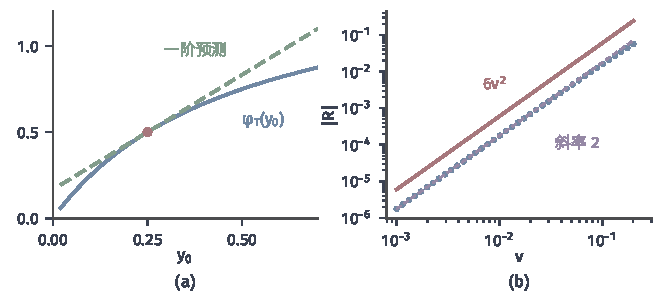
\includegraphics[width=112mm]{figures/06-differential-equations/01-ordinary-differential-equations/matplotlib/odesens-first-order/figure.pdf}
  \caption{Logistic方程的一阶预测，$T=\ln3$。(a)解映射$\varphi_T$（蓝）与红点处的一阶预测$\tfrac12+\tfrac43(y_0-\tfrac14)$（绿虚线）。(b)余项$\lvert R\rvert$随$v$的变化（蓝点），红线是上界$6v^2$，紫色虚线是斜率为$2$的参考线。}
  \label{fig:odesens-first-order}
\end{BookInlineFigure}

\subsection{初值导数}
\label{sec:odesens-initial-derivative}

只改变初值时$\bm{w}=\bm{0}$，变分方程齐次，解对$\bm{v}$线性。把$\bm{v}$依次取为$\mathbb{R}^{n}$的标准基，所得$n$个解排成一个矩阵，也就是解对初始状态的Jacobian矩阵
\begin{equation}
 \bm{S}(t)=\frac{\partial\bm{x}(t;\bm{x}_0)}{\partial\bm{x}_0}\in\mathbb{R}^{n\times n}.
 \label{eq:odesens-initial-jacobian}
\end{equation}
由式~\eqref{eq:odesens-variational}，它满足以单位矩阵为初值的线性系统
\begin{equation}
 \dot{\bm{S}}=\bm{A}(t)\bm{S},\qquad \bm{S}(t_0)=\bm{I}.
 \label{eq:odesens-initial-variational}
\end{equation}

这正是第~\ref{chap:linear-differential-systems}章的状态转移矩阵的定义方程。那里证明了$\bm{\Phi}(t,s)$对$t$满足该线性系统、$\bm{\Phi}(s,s)=\bm{I}$，并满足复合关系$\bm{\Phi}(t,s)\bm{\Phi}(s,r)=\bm{\Phi}(t,r)$。因此$\bm{S}(t)=\bm{\Phi}(t,t_0)$，只是这里的$\bm{A}(t)$来自沿解的线性化，$\bm{\Phi}$依赖于所选的轨迹。

\paragraph{水面上的小木棍}
想象在水流中放一根极短的小木棍，一端在参考点$\bm{x}_0$，另一端在$\bm{x}_0+\bm{v}$。水流带着小木棍前进，同时拉长、压短并转动它。$\bm{z}(t)=\bm{S}(t)\bm{v}$就是$t$时刻的小木棍。对应关系是：水流是右端$\bm{f}$，小木棍是切向量，$\bm{A}(t)$描述当前位置附近水流的局部拉伸与旋转。类比到有限长度就失效了，长木棍会弯曲，而$\bm{z}$永远是直的箭头。

把$\bm{S}(t)$作奇异值分解$\bm{S}=\bm{U}\bm{\Sigma}\bm{V}^{\top}$。单位球面上的初值方向被映成椭球面，最大奇异值$\sigma_{\max}$是一阶下最坏的放大倍数，相应的$\bm{V}$的列是最敏感的初值方向，$\bm{U}$的列是响应的方向。

\begin{example}[可以手算的二维系统]
\label{ex:odesens-planar}
考虑
\[
 \dot{x}_1=-x_1,\qquad \dot{x}_2=x_2+x_1^2,
\]
初值$(1,0)$。第一个方程给出$x_1(t)=\mathrm{e}^{-t}$，沿解的线性化系数是
\[
 \bm{A}(t)=\begin{bmatrix}-1&0\\2\mathrm{e}^{-t}&1\end{bmatrix}.
\]

按列解式~\eqref{eq:odesens-initial-variational}。第二列满足$\dot{s}_{1,2}=-s_{1,2}$、$\dot{s}_{2,2}=2\mathrm{e}^{-t}s_{1,2}+s_{2,2}$，初值$(0,1)$，于是
\[
 s_{1,2}=0,\qquad s_{2,2}=\mathrm{e}^{t}.
\]
第一列初值为$(1,0)$，由第一个方程得$s_{1,1}=\mathrm{e}^{-t}$，代入第二个方程，
\[
 \dot{s}_{2,1}=s_{2,1}+2\mathrm{e}^{-2t},\qquad s_{2,1}(0)=0.
\]

乘以积分因子$\mathrm{e}^{-t}$，得
\[
 \frac{\mathrm{d}}{\mathrm{d}t}\bigl(\mathrm{e}^{-t}s_{2,1}\bigr)=2\mathrm{e}^{-3t},
\]
积分后得到
\[
 s_{2,1}(t)=\tfrac23\bigl(\mathrm{e}^{t}-\mathrm{e}^{-2t}\bigr).
\]
取$t=\ln2$，参考解到达$(1/2,\,7/12)$，
\[
 \bm{S}(\ln2)=\begin{bmatrix}1/2&0\\7/6&2\end{bmatrix}.
\]

这个方程能显式求解，可以用来核对：从$(a,b)$出发，
\[
 x_1=a\mathrm{e}^{-t},\qquad x_2=\bigl(b+a^2/3\bigr)\mathrm{e}^{t}-\bigl(a^2/3\bigr)\mathrm{e}^{-2t}.
\]
对$(a,b)$在$(1,0)$处求导，结果与上式相同。$\bm{S}(\ln2)$的奇异值是$2.330$与$0.429$，最大奇异值比特征值$2$更大，这个差别来自$\bm{S}$非对称带来的转向。
\end{example}

图~\ref{fig:odesens-tangent-transport}把例~\ref{ex:odesens-planar}画了出来。红色小圆的两根基向量被$\bm{S}(\ln2)$带到蓝色箭头：$(1,0)$方向既缩短又转向，$(0,1)$方向被拉长两倍。半径$0.4$并不算小，真实的像（蓝色区域）和线性预测的椭圆（绿色虚线）已有肉眼可见的差别。

\begin{BookInlineFigure}
  \centering
  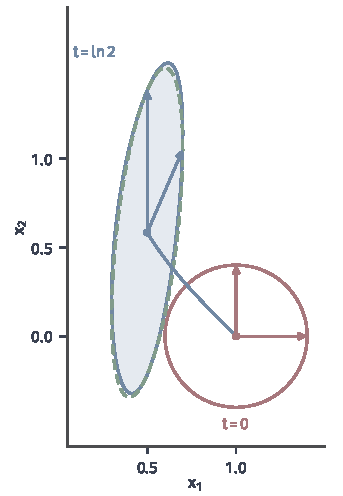
\includegraphics[width=58mm]{figures/06-differential-equations/01-ordinary-differential-equations/matplotlib/odesens-tangent-transport/figure.pdf}
  \caption{小圆随流的变形。方程为$\dot{x}_1=-x_1$，$\dot{x}_2=x_2+x_1^2$。红圆是$t=0$时以$(1,0)$为心、半径$0.4$的圆，蓝线是圆心的轨迹，浅蓝区域是$t=\ln2$时圆的真实像，绿色虚线是线性预测$\bm{x}(t)+\bm{S}(t)\bm{v}$的椭圆。红箭头是两根基向量，蓝箭头是它们在$\bm{S}(\ln2)$下的像。}
  \label{fig:odesens-tangent-transport}
\end{BookInlineFigure}

\paragraph{沿轨迹方向的导数}
自治方程有一个不用解方程就知道的解。对$\bm{f}(\bm{x}(t))$关于$t$求导，并用$\dot{\bm{x}}=\bm{f}(\bm{x})$，得到
\[
 \frac{\mathrm{d}}{\mathrm{d}t}\bm{f}(\bm{x}(t))=\bm{A}(t)\bm{f}(\bm{x}(t)).
\]
所以$\bm{f}(\bm{x}(t))$满足齐次变分方程，初值是$\bm{f}(\bm{x}_0)$。由线性方程的唯一性，
\begin{equation}
 \bm{S}(t)\,\bm{f}(\bm{x}_0)=\bm{f}(\bm{x}(t)).
 \label{eq:odesens-tangent-flow}
\end{equation}
含义是：把初值沿轨迹挪一点，只相当于把时间起点平移，$t$时刻的解也沿轨迹挪一点。

标量情形下，当$f(x_0)\neq0$时，式~\eqref{eq:odesens-tangent-flow}直接给出$S(t)=f(x(t))/f(x_0)$。在Logistic方程上，
\[
 S(\ln3)=\frac{\tfrac12\cdot\tfrac12}{\tfrac14\cdot\tfrac34}=\frac43,
\]
与例~\ref{ex:odesens-first-order}的积分结果一致。再继续到$t=2\ln3$，$x$从$1/2$增长到$3/4$，这一段的放大倍数是$(3/16)/(1/4)=3/4$，全程是$\tfrac43\cdot\tfrac34=1$，放大和压缩恰好抵消，这正是复合关系$\bm{\Phi}(t,s)\bm{\Phi}(s,r)=\bm{\Phi}(t,r)$的一个实例。

\paragraph{增长的$\bm{S}$不等于发散的轨迹}
Jacobian矩阵增长并不说明解跑远了。无阻尼摆$\dot{q}=p$、$\dot{p}=-\sin q$的轨道是封闭曲线，但周期依赖振幅。两条相邻轨道相位差随时间线性累积，$\bm{S}$的范数因而线性增长，见图~\ref{fig:odesens-pendulum-growth}。这里的增长来自相位的错开，不是轨道的分离，而轨迹全程有界。这再次说明，有限时间的一阶响应和长期行为是不同的问题。

\begin{BookInlineFigure}
  \centering
  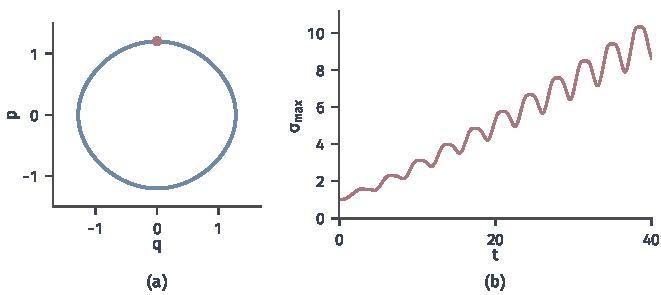
\includegraphics[width=112mm]{figures/06-differential-equations/01-ordinary-differential-equations/matplotlib/odesens-pendulum-growth/figure.pdf}
  \caption{无阻尼摆的初值Jacobian矩阵。(a)从红点$(q,p)=(0,1.2)$出发的封闭轨道。(b)式~\eqref{eq:odesens-initial-variational}数值积分得到的最大奇异值$\sigma_{\max}(t)$，在振荡中近似线性增长，$t=40$内从$1$升到约$10$，而轨道始终有界。}
  \label{fig:odesens-pendulum-growth}
\end{BookInlineFigure}

\subsection{参数导数}
\label{sec:odesens-parameter-derivative}

现在让参数变化。先取有限维参数$\bm{\theta}\in\mathbb{R}^{p}$，初值也可能依赖参数，写成$\bm{x}_0(\bm{\theta})$。把$\bm{w}$取遍标准基，方向导数排成矩阵
\begin{equation}
 \bm{P}(t)=\frac{\partial\bm{x}(t;\bm{\theta})}{\partial\bm{\theta}}\in\mathbb{R}^{n\times p}.
 \label{eq:odesens-parameter-jacobian}
\end{equation}
在式~\eqref{eq:odesens-variational}中$\bm{v}=(\partial_{\bm{\theta}}\bm{x}_0)\bm{w}$，于是$\bm{P}$满足
\begin{equation}
 \dot{\bm{P}}=\bm{A}(t)\bm{P}+\bm{B}(t),\qquad \bm{P}(t_0)=\partial_{\bm{\theta}}\bm{x}_0(\bm{\theta}).
 \label{eq:odesens-parameter-variational}
\end{equation}
与初值导数相比，多了非齐次项$\bm{B}(t)$：参数改变时，每一时刻的变化率都被额外推了一下。

这个线性方程的解由第~\ref{chap:linear-differential-systems}章的常数变易公式给出：
\begin{equation}
 \bm{P}(t)=\bm{\Phi}(t,t_0)\,\partial_{\bm{\theta}}\bm{x}_0+\int_{t_0}^{t}\bm{\Phi}(t,s)\bm{B}(s)\,\mathrm{d}s.
 \label{eq:odesens-parameter-formula}
\end{equation}
第一项是初值本身对参数的依赖，第二项是时刻$s$对变化率的推动再传播到$t$。结构和Gronwall上界完全对应，只是把放大因子的上界换成了真实的传播矩阵。

\begin{example}[增长率的导数]
\label{ex:odesens-parameter-derivative}
对$\dot{x}=\theta x(1-x)$，$\theta=1$，$x_0=1/4$，系数是
\[
 A(t)=1-2x(t),\qquad B(t)=x(t)(1-x(t)).
\]
初值不依赖参数，所以$P(0)=0$。式~\eqref{eq:odesens-parameter-variational}是$\dot{P}=(1-2x)P+x(1-x)$。

猜测$P=t\,x(1-x)$，即$P=tf(x)$，代入验证。由$\frac{\mathrm{d}}{\mathrm{d}t}f(x)=(1-2x)f(x)$，得到
\[
 \dot{P}=f(x)+t(1-2x)f(x)=x(1-x)+(1-2x)P,
\]
满足方程，且$P(0)=0$。这个结果也可以这样理解：解依赖$\theta t$，改变$\theta$相当于改变时间尺度。

在$t=\ln3$处，$x=1/2$，$P(\ln3)=\tfrac14\ln3\approx0.2747$。$\theta$增加$0.2$时，一阶预测的改变量是$0.0549$，例~\ref{ex:odesens-parameter-bound}中的真实差是$0.0547$，而Gronwall上界是$0.0901$。

若初值也依赖参数，比如$x_0(\theta)=\theta/4$，则$\partial_\theta x_0=1/4$，由式~\eqref{eq:odesens-parameter-formula}，
\[
 P(\ln3)=\frac43\cdot\frac14+\frac14\ln3\approx0.3333+0.2747=0.6080.
\]
前一项用了初值导数$S(\ln3)=4/3$。
\end{example}

图~\ref{fig:odesens-parameter-derivative}画出了$P(t)$。参数的影响在$x$中等时最大，$x$接近$0$或$1$时增长率的具体数值几乎不起作用。绿点是有限差分，它与变分方程的解重合。

\begin{BookInlineFigure}
  \centering
  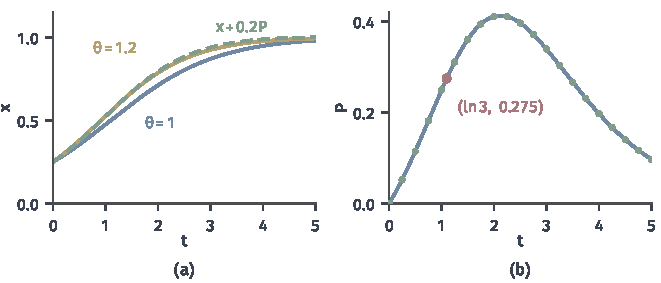
\includegraphics[width=112mm]{figures/06-differential-equations/01-ordinary-differential-equations/matplotlib/odesens-parameter-derivative/figure.pdf}
  \caption{参数导数。方程$\dot{x}=\theta x(1-x)$，$x_0=1/4$。(a)$\theta=1$（蓝）、$\theta=1.2$（黄）的解，绿色虚线是一阶预测$x+0.2P$。(b)$P(t)$的变分方程解（蓝）与有限差分（绿点），红点是$t=\ln3$处的值。}
  \label{fig:odesens-parameter-derivative}
\end{BookInlineFigure}

\paragraph{参数化的输入}
输入是一个函数，自由度无穷多。常见的做法是用有限个参数表示它，比如$\bm{g}(t)=\bm{g}(t;\bm{\theta})$，然后归入上面的计算。右端写成$\bm{f}(t,\bm{x},\bm{g}(t;\bm{\theta}))$，由链式法则，
\begin{equation}
 \bm{B}(t)=\partial_{\bm{g}}\bm{f}\bigl(t,\bm{x}(t),\bm{g}(t;\bm{\theta})\bigr)\,\partial_{\bm{\theta}}\bm{g}(t;\bm{\theta}).
 \label{eq:odesens-input-derivative}
\end{equation}
其余不变。定理~\ref{thm:odesens-differentiable}对$t$只要求可测，$\partial_{\bm{\theta}}\bm{g}$可以有跳变。

考虑$\dot{x}=-x+g(t)$，$x_0=0$，$t\in[0,2]$，$g$在$[0,1)$上取$\theta_1$，在$[1,2)$上取$\theta_2$，这里取$\theta_1=1$、$\theta_2=2$。此时$A=-1$，$\bm{B}(t)$在两段上分别是$(1,0)$与$(0,1)$，于是$P_j$分别解$\dot{P}_j=-P_j+B_j$。直接积分，
\[
 P_1(2)=\mathrm{e}^{-1}(1-\mathrm{e}^{-1})\approx0.2325,\qquad
 P_2(2)=1-\mathrm{e}^{-1}\approx0.6321.
\]
较早的输入经历了$\mathrm{e}^{-1}$的衰减，对末态的影响较小，图~\ref{fig:odesens-input-basis}(b)的折点就发生在切换时刻。

\begin{BookInlineFigure}
  \centering
  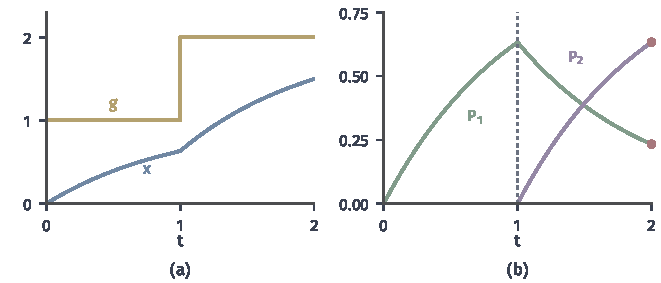
\includegraphics[width=112mm]{figures/06-differential-equations/01-ordinary-differential-equations/matplotlib/odesens-input-basis/figure.pdf}
  \caption{分段常值输入的参数导数。方程$\dot{x}=-x+g$，$x_0=0$。(a)输入$g$（黄）与解$x$（蓝），$\theta=(1,2)$。(b)参数导数$P_1$（绿）、$P_2$（紫），灰色虚线是切换时刻$t=1$，红点是$t=2$时的值。}
  \label{fig:odesens-input-basis}
\end{BookInlineFigure}

\section{解的流映射}
\label{sec:odesens-flow}

到现在为止我们盯着一条解和它附近的解。换一个视角：固定起止时刻，让所有初始状态同时运动。方向场上每一点都顺流而下，整个状态空间被搬动了一段。这个“搬动”本身是一个映射，前面得到的初值依赖、Jacobian矩阵都成为它的性质。

本节设$\bm{D}\subseteq\mathbb{R}\times\mathbb{R}^{n}$开，$\bm{f}:\bm{D}\to\mathbb{R}^{n}$连续，且$\partial_{\bm{x}}\bm{f}$在$\bm{D}$上存在并连续，这样过$\bm{D}$中每点的最大解都存在且唯一。时间可测时，把$\bm{f}$的条件换成定理~\ref{thm:odesens-differentiable}的条件，并把涉及时间导数的结论理解为几乎处处成立。

\begin{definition}[流映射]
\label{def:odesens-flow}
对时刻$s,t$，记$\bm{D}_{s,t}$为满足下述条件的$\bm{x}\in\mathbb{R}^{n}$的集合：$(s,\bm{x})\in\bm{D}$，且过$(s,\bm{x})$的最大解在时刻$t$有定义。在$\bm{D}_{s,t}$上定义\term{流映射}（flow map）
\begin{equation}
 \bm{\varphi}_{s,t}(\bm{x})=\text{过}(s,\bm{x})\text{的最大解在时刻}\ t\ \text{的值}.
 \label{eq:odesens-flow}
\end{equation}
\end{definition}

记号$\bm{\varphi}_{s,t}$保留了起止两个时刻。$\bm{D}_{s,t}$可能是真子集，甚至是空集，因为有些解活不到$t$。由定理~\ref{thm:odesens-local-lipschitz}，$\bm{D}_{s,t}$是开集，$\bm{\varphi}_{s,t}$在其上局部Lipschitz；由定理~\ref{thm:odesens-differentiable}，它连续可微，Jacobian矩阵是沿相应解的状态转移矩阵，
\begin{equation}
 \mathrm{D}\bm{\varphi}_{s,t}(\bm{x})=\bm{\Phi}(t,s).
 \label{eq:odesens-flow-jacobian}
\end{equation}
图~\ref{fig:odesens-flow-domain}是$\dot{x}=x^2$的流映射，它的定义域随$t$收缩。

\begin{BookInlineFigure}
  \centering
  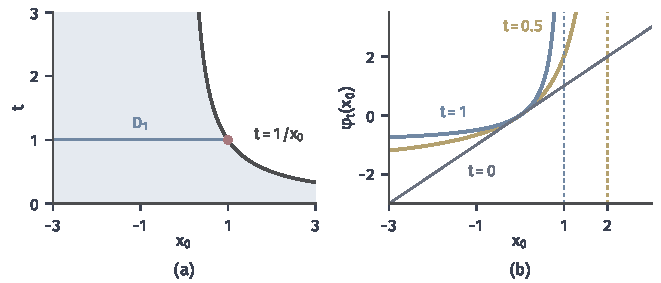
\includegraphics[width=112mm]{figures/06-differential-equations/01-ordinary-differential-equations/matplotlib/odesens-flow-domain/figure.pdf}
  \caption{流映射的定义域依赖时间。方程$\dot{x}=x^2$，$\varphi_t(x)=x/(1-tx)$。(a)浅蓝区域是$\{(x_0,t):t\geq0,\ tx_0<1\}$，深灰线是爆炸曲线$t=1/x_0$，蓝色水平线是$t=1$时的定义域$\bm{D}_1=(-\infty,1)$。(b)$\varphi_t$的图像，$t=0$是恒等映射（灰），$t=0.5$（黄）、$t=1$（蓝）在虚线处趋于无穷。}
  \label{fig:odesens-flow-domain}
\end{BookInlineFigure}

\subsection{局部可逆性}
\label{sec:odesens-flow-inverse}

解在唯一性条件下不会分叉也不会合并。所以从$s$走到$r$再走到$t$，应当等于直接走到$t$；从$s$走到$t$再走回来，应当回到原处。这是流映射的两条代数规则，图~\ref{fig:odesens-flow-composition}是它们的示意。

\begin{BookInlineFigure}
  \centering
  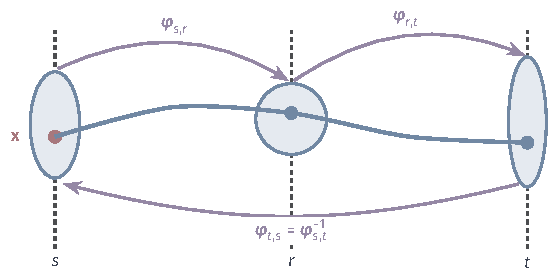
\includegraphics[width=93.4mm]{figures/06-differential-equations/01-ordinary-differential-equations/tikz/odesens-flow-composition/figure.pdf}
  \caption{流映射的复合与逆。三条虚线是时刻$s,r,t$上的状态空间，浅蓝区域是一小块初值及其像，蓝线是过红点的解。上方两个映射相继作用等于$\bm{\varphi}_{s,t}$，下方的映射$\bm{\varphi}_{t,s}$把终点送回起点。}
  \label{fig:odesens-flow-composition}
\end{BookInlineFigure}

\begin{theorem}[流映射的复合与局部可逆性]
\label{thm:odesens-flow}
在本节的条件下：
\begin{enumerate}
 \item 对$(s,\bm{x})\in\bm{D}$，有$\bm{\varphi}_{s,s}(\bm{x})=\bm{x}$；
 \item 若$\bm{x}\in\bm{D}_{s,r}$且$\bm{\varphi}_{s,r}(\bm{x})\in\bm{D}_{r,t}$，则$\bm{x}\in\bm{D}_{s,t}$，且
 \begin{equation}
  \bm{\varphi}_{r,t}\bigl(\bm{\varphi}_{s,r}(\bm{x})\bigr)=\bm{\varphi}_{s,t}(\bm{x});
  \label{eq:odesens-flow-composition}
 \end{equation}
 \item $\bm{\varphi}_{s,t}:\bm{D}_{s,t}\to\bm{D}_{t,s}$是$C^1$双射，逆映射是$\bm{\varphi}_{t,s}$，且Jacobian矩阵处处可逆，
 \begin{equation}
  \mathrm{D}\bm{\varphi}_{t,s}\bigl(\bm{\varphi}_{s,t}(\bm{x})\bigr)=\bigl[\mathrm{D}\bm{\varphi}_{s,t}(\bm{x})\bigr]^{-1}.
  \label{eq:odesens-flow-inverse}
 \end{equation}
\end{enumerate}
\end{theorem}

\begin{proof}
第一条是定义。

第二条用唯一性。过$(s,\bm{x})$的最大解在时刻$r$的值是$\bm{\varphi}_{s,r}(\bm{x})$，所以它也是过$(r,\bm{\varphi}_{s,r}(\bm{x}))$的解。由最大解的唯一性，这两条最大解相同。后者在$t$有定义，前者也就在$t$有定义，两边的值相等。

第三条是第二条的特例。设$\bm{x}\in\bm{D}_{s,t}$，$\bm{y}=\bm{\varphi}_{s,t}(\bm{x})$。过$(t,\bm{y})$的最大解就是过$(s,\bm{x})$的最大解，它在$s$有定义且值为$\bm{x}$，所以$\bm{y}\in\bm{D}_{t,s}$，且$\bm{\varphi}_{t,s}(\bm{y})=\bm{x}$。交换$s,t$得到另一个方向。两个映射都是$C^1$的，对恒等映射$\bm{\varphi}_{t,s}\circ\bm{\varphi}_{s,t}$用链式法则，就得到式~\eqref{eq:odesens-flow-inverse}。
\end{proof}

这里没有用到反函数定理，逆映射是由“反向求解”直接造出来的，并且在整个$\bm{D}_{s,t}$上有定义，不只在一点附近。之所以仍称为局部可逆性，是因为$\bm{D}_{s,t}$通常不是整个空间，定理并不假定解全局存在。

\paragraph{自治方程与单参数局部流}
当$\bm{f}$不显含时间时，若$\bm{x}(t)$是解，平移后的$\bm{x}(t+c)$也是解。于是$\bm{\varphi}_{s,t}$只依赖时长$t-s$，记$\bm{\varphi}_{t}=\bm{\varphi}_{0,t}$。式~\eqref{eq:odesens-flow-composition}变成
\begin{equation}
 \bm{\varphi}_{t}\circ\bm{\varphi}_{r}=\bm{\varphi}_{t+r}.
 \label{eq:odesens-local-flow}
\end{equation}
等式在式~\eqref{eq:odesens-flow-composition}的定义域条件下成立，所以$\{\bm{\varphi}_t\}$称为\term{单参数局部流}（local one-parameter flow）。若所有解全局存在，它才是定义在整个空间上的单参数群。

对$\dot{x}=x^2$，$\varphi_t(x)=x/(1-tx)$，直接代入，
\[
 \varphi_t\bigl(\varphi_r(x)\bigr)=\frac{x/(1-rx)}{1-tx/(1-rx)}=\frac{x}{1-(t+r)x}=\varphi_{t+r}(x),
\]
要求$rx<1$且$tx/(1-rx)<1$。当$t,r>0$时，这等价于$(t+r)x<1$；$\varphi_{-t}$是$\varphi_t$在定义域上的逆。

非自治方程不能这样简写。对$\dot{x}=tx$，$\varphi_{s,t}(x)=x\,\mathrm{e}^{(t^2-s^2)/2}$。从$0$走到$1$乘以$\mathrm{e}^{1/2}$，再用同一规律“走一个单位时间”乘以$\mathrm{e}^{1/2}$，得到的$\mathrm{e}$并不等于从$0$到$2$的倍数$\mathrm{e}^{2}$。第二段时间的起点是$1$，规律已经变了，所以必须记下起止两个时刻。

\paragraph{没有唯一性时会怎样}
可逆性来自轨道不合并。方程$\dot{x}=-2\,\mathrm{sgn}(x)\sqrt{\lvert x\rvert}$在$x=0$处不Lipschitz。正向解唯一：右端单调递减，式~\eqref{eq:odesens-one-sided}成立且$\mu=0$，由引理~\ref{lem:odesens-one-sided}，两条解的距离不增，所以正向唯一。解是
\[
 x(t)=\mathrm{sgn}(x_0)\bigl(\max\{\sqrt{\lvert x_0\rvert}-t,\,0\}\bigr)^2.
\]

所有$\lvert x_0\rvert\leq t^2$的轨道在时刻$t$都已并入$0$，见图~\ref{fig:odesens-merging}。$\varphi_1$把整个$[-1,1]$压成一点，不是单射，没有逆映射，这正是反向解不唯一的表现。

\begin{BookInlineFigure}
  \centering
  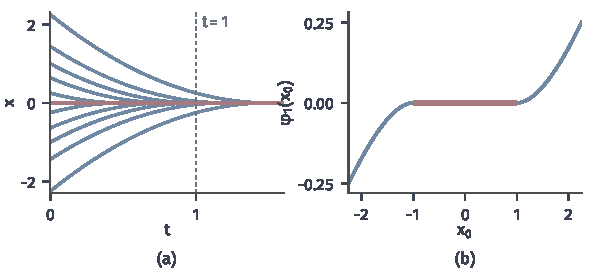
\includegraphics[width=100mm]{figures/06-differential-equations/01-ordinary-differential-equations/matplotlib/odesens-merging/figure.pdf}
  \caption{轨道合并破坏可逆性。方程$\dot{x}=-2\,\mathrm{sgn}(x)\sqrt{\lvert x\rvert}$。(a)各初值的轨道在有限时间并入红色的零解。(b)$t=1$时的解映射，红色线段$[-1,1]$被压成一点。}
  \label{fig:odesens-merging}
\end{BookInlineFigure}

\subsection{体积变化}
\label{sec:odesens-volume}

流映射把一小块初始区域搬到别处，体积会变吗？线性映射的体积倍数是行列式的绝对值，而流映射在一小块上近似线性，Jacobian矩阵是$\bm{S}(t)$。于是要看的是$J(t)=\det\bm{S}(t)$怎样随时间变化。

\paragraph{直观}
考虑很短的时间$h$，由式~\eqref{eq:odesens-initial-variational}有$\bm{S}(t+h)\approx(\bm{I}+h\bm{A}(t))\bm{S}(t)$。而
\[
 \det(\bm{I}+h\bm{A})=1+h\operatorname{tr}\bm{A}+O(h^2),
\]
所以每一小段时间内体积的相对变化率是$\operatorname{tr}\bm{A}$，也就是右端的散度。放在水流的图景中，散度是某点处水流的“膨胀率”：散度为正的地方，流体微团在膨胀。把这个观察写成精确的等式，就是\term{Liouville公式}（Liouville formula）。

\begin{lemma}[Liouville公式]
\label{lem:odesens-liouville}
设$\bm{S}$满足式~\eqref{eq:odesens-initial-variational}，其中$\bm{A}$可积。则$J=\det\bm{S}$绝对连续，几乎处处满足$\dot{J}=\operatorname{tr}\bm{A}(t)\,J$，于是
\begin{equation}
 J(t)=\exp\int_{t_0}^{t}\operatorname{tr}\bm{A}(s)\,\mathrm{d}s>0.
 \label{eq:odesens-liouville}
\end{equation}
\end{lemma}

\begin{proof}
行列式是矩阵元素的多项式，$\bm{S}$绝对连续，所以$J$绝对连续。矩阵函数的微分给出
\[
 \mathrm{d}\det{}_{\bm{S}}(\bm{E})=\operatorname{tr}\bigl(\operatorname{adj}(\bm{S})\bm{E}\bigr),
\]
这个公式对奇异矩阵也成立，可参考\BookChapterRef{chap:matrix-differentiation}{卷二第21章“矩阵函数的微分”}。代入$\dot{\bm{S}}=\bm{A}\bm{S}$，
\[
 \dot{J}=\operatorname{tr}\bigl(\operatorname{adj}(\bm{S})\bm{A}\bm{S}\bigr).
\]

用迹的循环性，再用$\bm{S}$与其古典伴随的乘积等于$\det(\bm{S})\bm{I}$，
\[
 \dot{J}=\operatorname{tr}\bigl(\bm{A}\bm{S}\operatorname{adj}(\bm{S})\bigr)=\operatorname{tr}(\bm{A})\,J.
\]
这是标量线性方程，$J(t_0)=1$，解就是式~\eqref{eq:odesens-liouville}。
\end{proof}

沿解，$\operatorname{tr}\bm{A}(t)$正是右端在$(t,\bm{x}(t))$处的散度$\nabla\cdot\bm{f}$，这里的散度只对状态变量求。式~\eqref{eq:odesens-liouville}中$J>0$说明流映射保持定向，也就不会出现把区域翻折的情况。

三个手算例子可以用来核对。常系数线性方程$\dot{\bm{x}}=\bm{A}\bm{x}$有
\[
 \det\mathrm{e}^{t\bm{A}}=\mathrm{e}^{t\operatorname{tr}\bm{A}}.
\]
例~\ref{ex:odesens-planar}的散度是$-1+1=0$，相应的行列式是$\tfrac12\cdot2=1$。Logistic方程是一维的，“体积”就是长度，放大倍数$\exp\int(1-2x)\,\mathrm{d}t$等于$4/3$，与$S(\ln3)$相同。

\begin{theorem}[体积变化公式]
\label{thm:odesens-volume}
在本节的条件下，设$\bm{W}\subseteq\bm{D}_{s,t}$是可测集。则
\begin{equation}
 \operatorname{vol}\bigl(\bm{\varphi}_{s,t}(\bm{W})\bigr)=\int_{\bm{W}}\exp\Bigl(\int_{s}^{t}\nabla\cdot\bm{f}\bigl(r,\bm{\varphi}_{s,r}(\bm{x})\bigr)\,\mathrm{d}r\Bigr)\mathrm{d}\bm{x}.
 \label{eq:odesens-volume}
\end{equation}
特别地，若$\bm{f}$的定义域$\bm{D}$上$\nabla\cdot\bm{f}\equiv0$，则流映射保持体积。反过来，若流映射对任意$s,t$和任意小球都保持体积，则$\nabla\cdot\bm{f}\equiv0$。
\end{theorem}

\begin{proof}
由定理~\ref{thm:odesens-flow}，$\bm{\varphi}_{s,t}$是开集之间的$C^1$双射，且Jacobian矩阵可逆。换元公式给出
\[
 \operatorname{vol}\bigl(\bm{\varphi}_{s,t}(\bm{W})\bigr)=\int_{\bm{W}}\bigl\lvert\det\mathrm{D}\bm{\varphi}_{s,t}(\bm{x})\bigr\rvert\,\mathrm{d}\bm{x}.
\]
这个公式及测度论背景可参考\BookChapterRef{chap:pushforward-measures}{卷四第9章“推前测度”}。把式~\eqref{eq:odesens-flow-jacobian}、式~\eqref{eq:odesens-liouville}代入，即得式~\eqref{eq:odesens-volume}，绝对值因$J>0$可去。

散度恒为零时，被积函数恒为$1$，体积保持。反过来，设某点$(s,\bm{x})$处$\nabla\cdot\bm{f}>0$（负的情形相同）。由连续性，$(s,\bm{x})$附近散度为正，取小球$\bm{W}$和很短的时间，使轨道段留在这个邻域内，则式~\eqref{eq:odesens-volume}的指数中积分为正，体积严格增大，矛盾。
\end{proof}

定理的条件都起作用。解的唯一性保证$\bm{\varphi}_{s,t}$单射，否则换元公式就不再有意义，图~\ref{fig:odesens-merging}的压缩映射便是反例。$\bm{f}$关于状态$C^1$保证了$\mathrm{D}\bm{\varphi}$连续。结论仅对$\bm{W}\subseteq\bm{D}_{s,t}$成立，爆炸的解所在的点不在其中。

图~\ref{fig:odesens-volume-change}比较了三种流。例~\ref{ex:odesens-planar}的流把正方形拉成细长曲边四边形，面积不变。阻尼振子$\dot{q}=p$、$\dot{p}=-q-\tfrac12p$的散度是$-\tfrac12$，面积按$\mathrm{e}^{-t/2}$缩小，边长$0.5$的正方形面积$0.25$，$t=2$时为$0.25\,\mathrm{e}^{-1}\approx0.092$。

\begin{BookInlineFigure}
  \centering
  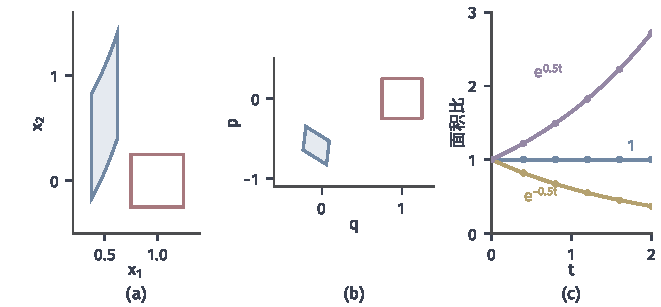
\includegraphics[width=112mm]{figures/06-differential-equations/01-ordinary-differential-equations/matplotlib/odesens-volume-change/figure.pdf}
  \caption{面积随流的变化。红框是初始正方形，浅蓝区域是它的像。(a)$\dot{x}_1=-x_1$、$\dot{x}_2=x_2+x_1^2$，$t=\ln2$，散度为零。(b)$\dot{q}=p$、$\dot{p}=-q-\tfrac12p$，$t=2$，散度为$-\tfrac12$。(c)面积比随时间的变化：线是式~\eqref{eq:odesens-liouville}，点是由多边形面积算出的数值；蓝、黄分别对应(a)(b)，紫色对应$\dot{\bm{x}}=\tfrac14\bm{x}$。}
  \label{fig:odesens-volume-change}
\end{BookInlineFigure}

\paragraph{沿轨迹的值与密度}
一块墨水随水流运动，某个粒子携带的值沿轨迹不变，而墨水的密度要随微团的伸缩改变，这是两件不同的事。设质量密度$p_s$在流映射下被推到$p_t$，质量守恒要求对任意$\bm{W}$有
\[
 \int_{\bm{\varphi}_{s,t}(\bm{W})}p_t(\bm{y})\,\mathrm{d}\bm{y}=\int_{\bm{W}}p_s(\bm{x})\,\mathrm{d}\bm{x}.
\]
左边用换元公式换回$\bm{x}$，比较被积函数，得到
\begin{equation}
 p_t\bigl(\bm{\varphi}_{s,t}(\bm{x})\bigr)=\frac{p_s(\bm{x})}{\det\mathrm{D}\bm{\varphi}_{s,t}(\bm{x})}.
 \label{eq:odesens-density}
\end{equation}
取对数并对$t$求导，由式~\eqref{eq:odesens-liouville}，沿轨迹有
\[
 \frac{\mathrm{d}}{\mathrm{d}t}\ln p_t\bigl(\bm{x}(t)\bigr)=-\nabla\cdot\bm{f}\bigl(t,\bm{x}(t)\bigr).
\]
膨胀的地方密度下降。

以Logistic方程为例。$x_0$在$[0.1,0.4]$上均匀分布，密度$p_0=10/3$。$T=\ln3$时，$x_0=1/4$被送到$1/2$，Jacobian是$4/3$，所以
\[
 p_T(1/2)=\frac{10/3}{4/3}=2.5.
\]
图~\ref{fig:odesens-density-push}对比了这个公式与样本直方图。右侧的$x_0$被拉伸得少，密度更高。式~\eqref{eq:odesens-density}是第~\ref{chap:transport-equations}章输运方程的基础，随机变量经可逆映射变换时的密度公式也是同一件事，可参考\BookChapterRef{chap:random-sampling-integration}{卷七第14章“随机采样与积分计算”}。

\begin{BookInlineFigure}
  \centering
  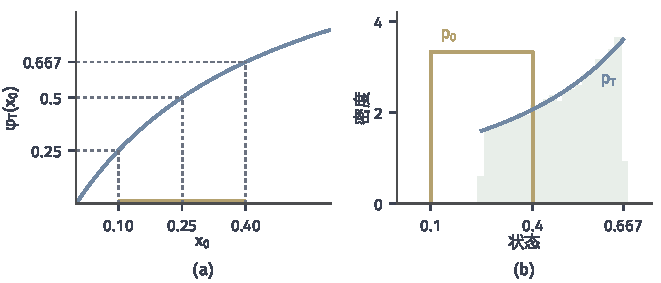
\includegraphics[width=112mm]{figures/06-differential-equations/01-ordinary-differential-equations/matplotlib/odesens-density-push/figure.pdf}
  \caption{流映射推动密度。方程$\dot{x}=x(1-x)$，$T=\ln3$。(a)流映射把黄色区间$[0.1,0.4]$送到$[0.25,0.667]$。(b)均匀密度$p_0$（黄）被推成$p_T$（蓝），绿色直方图来自$40000$个由固定种子生成的样本。}
  \label{fig:odesens-density-push}
\end{BookInlineFigure}

\subsection{Hamilton流}
\label{sec:odesens-hamilton}

有一类重要的方程，散度为零是结构带来的，不用逐个验证。力学系统的状态由位置$\bm{q}$和动量$\bm{p}$组成，运动由一个函数决定。摆的总能量是$H(q,p)=\tfrac12p^2+1-\cos q$，而摆的方程$\dot{q}=p$、$\dot{p}=-\sin q$恰好是
\[
 \dot{q}=\partial_pH,\qquad \dot{p}=-\partial_qH.
\]
这个形式可以推广。

\begin{definition}[Hamilton方程]
\label{def:odesens-hamilton}
设$H(t,\bm{q},\bm{p})$是定义在$\mathbb{R}\times\mathbb{R}^{m}\times\mathbb{R}^{m}$的开集上的函数，关于$t$连续，关于$(\bm{q},\bm{p})$二阶连续可微，且这些偏导数连续。称
\begin{equation}
 \dot{\bm{q}}=\nabla_{\bm{p}}H(t,\bm{q},\bm{p}),\qquad
 \dot{\bm{p}}=-\nabla_{\bm{q}}H(t,\bm{q},\bm{p})
 \label{eq:odesens-hamilton}
\end{equation}
为\term{Hamilton方程}（Hamilton's equations），$H$称为Hamilton函数（Hamiltonian），$(\bm{q},\bm{p})\in\mathbb{R}^{2m}$所在空间称为\term{相空间}（phase space），相应的流映射称为\term{Hamilton流}（Hamiltonian flow）。
\end{definition}

$H\in C^2$正好保证右端关于状态$C^1$，本节前面的结论全部适用。下面两条性质分别回答体积和能量。

\begin{theorem}[Hamilton流的体积与能量]
\label{thm:odesens-hamilton}
在定义~\ref{def:odesens-hamilton}的条件下，Hamilton流在其定义域内保持相空间体积（$H$可以显含时间）。若$H$还关于$t$连续可微，沿Hamilton方程的解有
\begin{equation}
 \frac{\mathrm{d}}{\mathrm{d}t}H\bigl(t,\bm{q}(t),\bm{p}(t)\bigr)=\partial_tH\bigl(t,\bm{q}(t),\bm{p}(t)\bigr).
 \label{eq:odesens-energy}
\end{equation}
特别地，$H$不显含时间时，$H$沿解不变。
\end{theorem}

\begin{proof}
相空间中的散度是
\[
 \nabla\cdot\bm{f}=\sum_{i=1}^{m}\Bigl(\frac{\partial}{\partial q_i}\frac{\partial H}{\partial p_i}-\frac{\partial}{\partial p_i}\frac{\partial H}{\partial q_i}\Bigr)=0,
\]
最后一步用了$H\in C^2$时混合偏导相等。由定理~\ref{thm:odesens-volume}，流保持体积。

由链式法则及式~\eqref{eq:odesens-hamilton}，
\[
 \frac{\mathrm{d}H}{\mathrm{d}t}=\partial_tH+\langle\nabla_{\bm{q}}H,\dot{\bm{q}}\rangle+\langle\nabla_{\bm{p}}H,\dot{\bm{p}}\rangle=\partial_tH+\langle\nabla_{\bm{q}}H,\nabla_{\bm{p}}H\rangle-\langle\nabla_{\bm{p}}H,\nabla_{\bm{q}}H\rangle.
\]
后两项相消，即得式~\eqref{eq:odesens-energy}。
\end{proof}

显含时间时，能量可以变化。受迫振子取$H=\tfrac12p^2+\tfrac12q^2-g(t)q$，方程是$\dot{q}=p$、$\dot{p}=-q+g(t)$，式~\eqref{eq:odesens-energy}的右端是$-\dot{g}(t)q$。取$g(t)=t$，$q(0)=0$，$p(0)=1$，解是$q=t$、$p=1$，代入$H$得
\[
 H(t,t,1)=\tfrac12+\tfrac12t^2-t^2=\tfrac12-\tfrac12t^2.
\]
其导数是$-t$，正好等于$-\dot{g}q=-t$。此时能量不守恒，但相空间体积仍然保持。

图~\ref{fig:odesens-hamilton-flow}是摆的相空间。在无阻尼情形下，半径$0.35$的圆被剪切成细长的月牙形，沿能量等值线运动，面积在$t=0,3,6$时都是$0.3848$。加上阻尼$\dot{p}=-\sin q-0.4p$后，方程不再是Hamilton方程，散度为$-0.4$，面积按$\mathrm{e}^{-0.4t}$缩小到$0.1159$与$0.0349$。

\begin{BookInlineFigure}
  \centering
  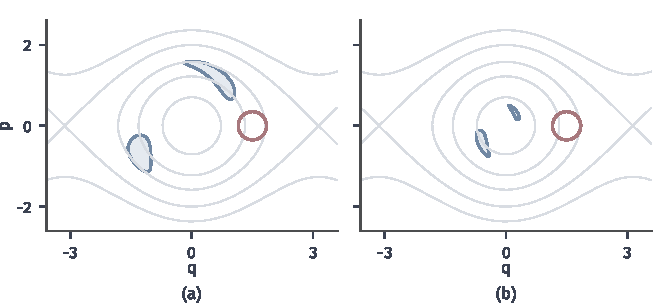
\includegraphics[width=112mm]{figures/06-differential-equations/01-ordinary-differential-equations/matplotlib/odesens-hamilton-flow/figure.pdf}
  \caption{摆的相空间。灰线是能量$H=\tfrac12p^2+1-\cos q$的等值线，红圆是初始区域，浅蓝区域是$t=3$和$t=6$时的像。(a)无阻尼，面积保持。(b)阻尼系数$0.4$，面积按$\mathrm{e}^{-0.4t}$收缩，区域离开能量等值线向内运动。}
  \label{fig:odesens-hamilton-flow}
\end{BookInlineFigure}

体积保持和能量守恒是两个不同的性质，互相不能推出，见表~\ref{tab:odesens-volume-energy}。

\begin{BookInlineTable}
  \centering
  \caption{体积保持与能量守恒的对比。“能量”指表中给定的函数。}
  \label{tab:odesens-volume-energy}
  \begin{tabular}{p{52mm}p{14mm}p{30mm}}
    \toprule
    系统 & 体积 & 能量 \\
    \midrule
    自治Hamilton方程 & 保持 & 守恒 \\
    显含时间的Hamilton方程 & 保持 & 按$\partial_tH$变化 \\
    阻尼摆 & 收缩 & $H$单调不增 \\
    $\dot{q}=(1+q^2)p$，$\dot{p}=-(1+q^2)q$ & 不保持 & $q^2+p^2$守恒 \\
    \bottomrule
  \end{tabular}
\end{BookInlineTable}

表中最后一行的散度是$2qp$，非零，但
\[
 \frac{\mathrm{d}}{\mathrm{d}t}(q^2+p^2)=2(1+q^2)(qp-pq)=0.
\]
这样的方程沿能量面运动，却不保持体积。

Hamilton流的这两条性质是后面几处的基础。第~\ref{chap:hamilton-jacobi-equations}章由Hamilton方程构造特征线，用它们重建场。构造采样提议时，流的可逆性和体积保持让接受概率的计算得以简化，可参考\BookChapterRef{chap:discrete-time-stochastic-processes}{卷九第3章“离散时间随机过程”}。两者都不说明解会靠拢，能量不变也不能推出渐近收敛。

\section{伴随方程}
\label{sec:odesens-adjoint}

设参数有$p$个，而我们只关心由解算出的一个数，比如终点状态的某个函数。用式~\eqref{eq:odesens-parameter-variational}求梯度，就要解一个$n\times p$的矩阵方程，相当于$p$个线性系统。$p$很大时这难以承受，而我们要的只是一个数对$p$个参数的导数。能不能只解一次方程？

\paragraph{主要思想}
设目标函数同时含终端项和沿途的运行项：
\begin{equation}
 J(\bm{\theta})=\psi\bigl(\bm{x}(T),\bm{\theta}\bigr)+\int_{t_0}^{T}\ell\bigl(t,\bm{x}(t),\bm{\theta}\bigr)\,\mathrm{d}t,
 \label{eq:odesens-objective}
\end{equation}
其中$\bm{x}$解$\dot{\bm{x}}=\bm{f}(t,\bm{x},\bm{\theta})$，$\bm{x}(t_0)=\bm{x}_0(\bm{\theta})$。沿方向$\bm{w}$求导，$\bm{z}=\bm{P}\bm{w}$解变分方程，得到
\[
 \mathrm{D}J[\bm{w}]=\langle\nabla_{\bm{x}}\psi,\bm{z}(T)\rangle+\langle\nabla_{\bm{\theta}}\psi,\bm{w}\rangle+\int_{t_0}^{T}\bigl(\langle\nabla_{\bm{x}}\ell,\bm{z}\rangle+\langle\nabla_{\bm{\theta}}\ell,\bm{w}\rangle\bigr)\,\mathrm{d}t.
\]
麻烦的是$\bm{z}$，每换一个$\bm{w}$都要重解。

解决办法来自一个恒等式。设$\bm{z}$解$\dot{\bm{z}}=\bm{A}\bm{z}$，$\bm{\lambda}$解$\dot{\bm{\lambda}}=-\bm{A}^{\top}\bm{\lambda}$，则
\[
 \frac{\mathrm{d}}{\mathrm{d}t}\langle\bm{\lambda},\bm{z}\rangle=\langle-\bm{A}^{\top}\bm{\lambda},\bm{z}\rangle+\langle\bm{\lambda},\bm{A}\bm{z}\rangle=0.
\]
配对$\langle\bm{\lambda},\bm{z}\rangle$沿时间不变。如果$\bm{\lambda}$在终点等于目标的梯度，那么
\[
 \langle\nabla\psi,\bm{z}(T)\rangle=\langle\bm{\lambda}(t_0),\bm{z}(t_0)\rangle.
\]
于是问题转移到了起点：$\bm{z}(t_0)$是已知的。代价是$\bm{\lambda}$的条件给在终点，要从$T$反向解回$t_0$，图~\ref{fig:odesens-adjoint-scheme}是这个结构的示意。

\begin{BookInlineFigure}
  \centering
  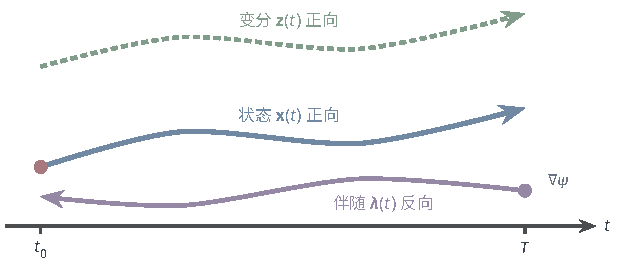
\includegraphics[width=105.2mm]{figures/06-differential-equations/01-ordinary-differential-equations/tikz/odesens-adjoint-scheme/figure.pdf}
  \caption{伴随计算的结构。状态$\bm{x}$从红色初值正向求解。变分$\bm{z}$（绿色虚线）也是正向的，每个方向都要解一次，伴随方法用不到它。伴随$\bm{\lambda}$（紫）从终点条件$\nabla\psi$出发反向求解，只解一次。配对$\langle\bm{\lambda},\bm{z}\rangle$在无运行项、无输入项时沿时间不变。}
  \label{fig:odesens-adjoint-scheme}
\end{BookInlineFigure}

一般情形多了非齐次项，只要在$\bm{\lambda}$的方程里补上运行项的梯度。在变分方程上演算，就得到下面的定理。

\begin{theorem}[伴随表示]
\label{thm:odesens-adjoint}
设$\bm{f}$满足定理~\ref{thm:odesens-differentiable}的条件，$\bm{x}_0(\bm{\theta})$、$\psi$连续可微，$\ell$对$t$可测、对$(\bm{x},\bm{\theta})$连续可微，且其导数在管道内被可积函数控制。设$\bm{A},\bm{B}$由式~\eqref{eq:odesens-coefficients}定义。令$\bm{\lambda}:[t_0,T]\to\mathbb{R}^{n}$是反向线性问题
\begin{equation}
 \dot{\bm{\lambda}}=-\bm{A}(t)^{\top}\bm{\lambda}-\nabla_{\bm{x}}\ell\bigl(t,\bm{x}(t),\bm{\theta}\bigr),\qquad
 \bm{\lambda}(T)=\nabla_{\bm{x}}\psi\bigl(\bm{x}(T),\bm{\theta}\bigr)
 \label{eq:odesens-adjoint}
\end{equation}
的解。则$J$在$\bm{\theta}$处可微，且
\begin{equation}
 \begin{aligned}
 \nabla J(\bm{\theta})={}&\nabla_{\bm{\theta}}\psi+\bigl[\partial_{\bm{\theta}}\bm{x}_0(\bm{\theta})\bigr]^{\top}\bm{\lambda}(t_0)\\
 &+\int_{t_0}^{T}\bigl[\bm{B}(t)^{\top}\bm{\lambda}(t)+\nabla_{\bm{\theta}}\ell\bigr]\,\mathrm{d}t.
 \end{aligned}
 \label{eq:odesens-adjoint-gradient}
\end{equation}
\end{theorem}

\begin{proof}
可微性由定理~\ref{thm:odesens-differentiable}、$\psi$的可微性以及该定理证明第四步那样的控制收敛论证得到，方向导数正是前面写出的$\mathrm{D}J[\bm{w}]$。式~\eqref{eq:odesens-adjoint}是系数可积的线性方程，在$[t_0,T]$上有唯一的绝对连续解。

设$\bm{z}$解方向$\bm{w}$的变分方程~\eqref{eq:odesens-variational}，起点取$(\partial_{\bm{\theta}}\bm{x}_0)\bm{w}$。计算配对的导数，$\bm{A}$的项相消，几乎处处有
\[
 \frac{\mathrm{d}}{\mathrm{d}t}\langle\bm{\lambda},\bm{z}\rangle=-\langle\nabla_{\bm{x}}\ell,\bm{z}\rangle+\langle\bm{\lambda},\bm{B}\bm{w}\rangle.
\]

从$t_0$到$T$积分，并代入$\bm{\lambda}(T)=\nabla_{\bm{x}}\psi$，移项得
\[
 \langle\nabla_{\bm{x}}\psi,\bm{z}(T)\rangle+\int_{t_0}^{T}\langle\nabla_{\bm{x}}\ell,\bm{z}\rangle\,\mathrm{d}t=\langle\bm{\lambda}(t_0),\bm{z}(t_0)\rangle+\int_{t_0}^{T}\langle\bm{\lambda},\bm{B}\bm{w}\rangle\,\mathrm{d}t.
\]
左边正是$\mathrm{D}J[\bm{w}]$中含$\bm{z}$的部分。代回$\mathrm{D}J[\bm{w}]$，右端对$\bm{w}$线性，读出系数就是式~\eqref{eq:odesens-adjoint-gradient}。
\end{proof}

称$\bm{\lambda}$为\term{伴随变量}（adjoint variable），式~\eqref{eq:odesens-adjoint}为\term{伴随方程}（adjoint equation）。式~\eqref{eq:odesens-adjoint-gradient}的各项对应目标导数的三个来源：含$\nabla_{\bm{\theta}}\psi$与$\nabla_{\bm{\theta}}\ell$的项是目标函数显含参数的部分；含$\bm{\lambda}(t_0)$的项是初值对参数的依赖；含$\bm{B}$的项是右端对参数的依赖。

\paragraph{$\bm{\lambda}$的含义}
无运行项时，比较式~\eqref{eq:odesens-adjoint}与式~\eqref{eq:odesens-initial-variational}，得到
\begin{equation}
 \bm{\lambda}(t)=\bm{\Phi}(T,t)^{\top}\nabla_{\bm{x}}\psi\bigl(\bm{x}(T)\bigr).
 \label{eq:odesens-adjoint-pullback}
\end{equation}
也就是说，$\bm{\lambda}(t)$是目标函数对时刻$t$状态的梯度：如果在时刻$t$把状态推动$\bm{v}$，目标函数的一阶变化是$\langle\bm{\lambda}(t),\bm{v}\rangle$。带运行项时含义相同，只是目标函数换成从$t$到$T$的累计。变分$\bm{z}$回答“推一下起点，后面怎么变”，伴随$\bm{\lambda}$回答“后面的目标，对前面每一刻有多敏感”，一个前传，一个后传。

\begin{example}[Logistic方程上的配对]
\label{ex:odesens-adjoint-logistic}
继续$\dot{x}=\theta x(1-x)$，$\theta=1$，$x_0=1/4$，$T=\ln3$，取$J=x(T)$，即$\psi(x)=x$，$\ell=0$。伴随方程是$\dot{\lambda}=-(1-2x)\lambda$，$\lambda(T)=1$。

记$f(x)=x(1-x)$。对$1/f(x(t))$求导，得到
\[
 \frac{\mathrm{d}}{\mathrm{d}t}\,\frac{1}{f(x)}=-\frac{1-2x}{f(x)}.
\]
所以$1/f(x(t))$满足伴随方程的齐次形式，配上终端条件，得
\[
 \lambda(t)=\frac{f(x(T))}{f(x(t))}.
\]
代入数据，$f(x(T))=1/4$，所以$\lambda(0)=\dfrac{1/4}{3/16}=\dfrac43$，这就是初值导数$S(T)$，与式~\eqref{eq:odesens-adjoint-pullback}一致。

对$\theta$的导数，$B(t)=f(x(t))$，所以
\[
 \lambda(t)B(t)=f(x(T))=\frac14\quad\text{（对所有}\ t\text{）}.
\]
积分得到$\partial_\theta J=\tfrac14\ln3\approx0.2747$，与例~\ref{ex:odesens-parameter-derivative}的$P(\ln3)$相同。
\end{example}

图~\ref{fig:odesens-adjoint-pairing}(a)中，$z=S(t)$从$1$升到$4/3$，$\lambda$从$4/3$降到$1$，乘积始终是$4/3$，这正是配对不变的数值表现。(b)显示伴随变量和被积函数的具体形状。

\begin{BookInlineFigure}
  \centering
  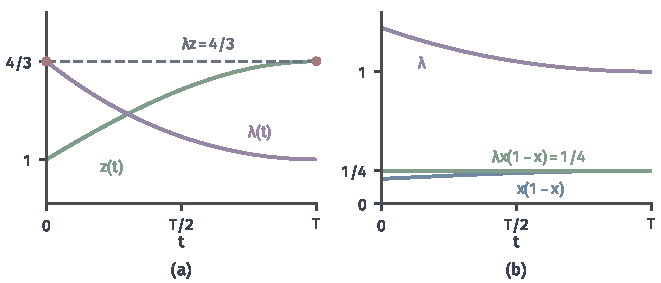
\includegraphics[width=112mm]{figures/06-differential-equations/01-ordinary-differential-equations/matplotlib/odesens-adjoint-pairing/figure.pdf}
  \caption{Logistic方程上的变分与伴随，$x_0=1/4$，$T=\ln3$，$J=x(T)$，数值积分得到。(a)前向的$z(t)=S(t)$（绿）与反向的$\lambda(t)$（紫），灰色虚线是乘积$\lambda z\equiv4/3$。红点是$\lambda(0)=z(T)=4/3$。(b)$\lambda$（紫）、$B=x(1-x)$（蓝）及其乘积（绿），乘积恒为$1/4$。}
  \label{fig:odesens-adjoint-pairing}
\end{BookInlineFigure}

\begin{example}[三个来源逐项核对]
\label{ex:odesens-adjoint-three}
取$\dot{x}=\theta x$，$x(0)=\theta$，$T=1$，
\[
 J(\theta)=\int_0^1\Bigl(x(t)+\frac12\theta^2\Bigr)\mathrm{d}t.
\]
解是$x=\theta\mathrm{e}^{\theta t}$，直接积分得$J=\mathrm{e}^{\theta}-1+\tfrac12\theta^2$，所以$J'(1)=\mathrm{e}+1$。

用伴随计算，取$\theta=1$。这里$\psi=0$，$\ell=x+\tfrac12\theta^2$，$A=1$，$B=x=\mathrm{e}^{t}$。伴随方程$\dot{\lambda}=-\lambda-1$、$\lambda(1)=0$的解是
\[
 \lambda(t)=\mathrm{e}^{1-t}-1.
\]

三项贡献依次是：
\[
 \begin{aligned}
 \text{初值：}&\ \partial_\theta x_0\,\lambda(0)=1\cdot(\mathrm{e}-1)=\mathrm{e}-1,\\
 \text{右端：}&\ \int_0^1\lambda B\,\mathrm{d}t=\int_0^1\bigl(\mathrm{e}-\mathrm{e}^{t}\bigr)\mathrm{d}t=1,\\
 \text{目标：}&\ \int_0^1\partial_\theta\ell\,\mathrm{d}t=\int_0^1\theta\,\mathrm{d}t=1.
 \end{aligned}
\]
相加得$\mathrm{e}+1$，与直接求导的结果相同。
\end{example}

\paragraph{计算过程}
下面把伴随方法写成计算过程，并同时在第~\ref{sec:odesens-parameter-derivative}节的分段输入例子上执行：$\dot{x}=-x+g(t)$，$x_0=0$，$T=2$，$g$在$[0,1)$、$[1,2)$上分别取$\theta_1=1$、$\theta_2=2$，目标是$J=\tfrac12x(2)^2$。

\needspace{6\baselineskip}
\paragraph{变量}
需要的量是：
\begin{itemize}
 \item 状态轨迹$\bm{x}(t)\in\mathbb{R}^{n}$，要保存下来或能够重新算出，供反向求解时使用；
 \item 伴随变量$\bm{\lambda}(t)\in\mathbb{R}^{n}$；
 \item 累积梯度$\bm{G}(t)\in\mathbb{R}^{p}$，表示$[t,T]$这段时间已经计入的梯度贡献。
\end{itemize}

\paragraph{初始化}
参数$\bm{\theta}$、初值$\bm{x}_0(\bm{\theta})$给定。例中$\bm{\theta}=(1,2)$，$x_0=0$，$\partial_{\bm{\theta}}x_0=\bm{0}$。

\needspace{6\baselineskip}
\paragraph{计算步骤}
\begin{enumerate}
 \item \emph{正向求解状态}，得到$\bm{x}(t)$，$t\in[t_0,T]$。例中逐段积分，
 \[
  x(1)=1-\mathrm{e}^{-1}=0.63212,\qquad x(2)=2+\bigl(x(1)-2\bigr)\mathrm{e}^{-1}=1.49679.
 \]

 \item \emph{设置终端条件}。令
 \[
  \bm{\lambda}(T)=\nabla_{\bm{x}}\psi(\bm{x}(T),\bm{\theta}),\qquad\bm{G}(T)=\bm{0}.
 \]
 例中$\lambda(2)=x(2)=1.49679$。

 \item \emph{反向求解伴随}。由式~\eqref{eq:odesens-adjoint}从$T$积到$t_0$，同时累积
 \[
  \dot{\bm{G}}=-\bigl[\bm{B}(t)^{\top}\bm{\lambda}(t)+\nabla_{\bm{\theta}}\ell\bigr].
 \]
 例中$A=-1$，无运行项，方程为$\dot{\lambda}=\lambda$，所以$\lambda(t)=x(2)\mathrm{e}^{t-2}$，
 \[
  \lambda(1)=0.55064,\qquad\lambda(0)=0.20257.
 \]

 \item \emph{合成梯度}。由式~\eqref{eq:odesens-adjoint-gradient}，
 \[
  \nabla J=\bm{G}(t_0)+\nabla_{\bm{\theta}}\psi+\bigl[\partial_{\bm{\theta}}\bm{x}_0\bigr]^{\top}\bm{\lambda}(t_0).
 \]
 例中$B$在$[0,1)$上为$(1,0)$，在$[1,2)$上为$(0,1)$，初值项为零，
 \[
  \partial_{\theta_1}J=\int_0^1\lambda\,\mathrm{d}t=0.34807,\qquad
  \partial_{\theta_2}J=\int_1^2\lambda\,\mathrm{d}t=0.94615.
 \]
\end{enumerate}

积分到$t_0$，计算结束。最终得到$\nabla J(1,2)=(0.34807,\,0.94615)$。用第~\ref{sec:odesens-parameter-derivative}节的$P_j(2)$核对，$\partial_{\theta_j}J=x(2)P_j(2)$，分别是$1.49679\times0.23254$与$1.49679\times0.63212$，结果相同。

图~\ref{fig:odesens-adjoint-gradient}把输入分成$20$段。一次反向积分给出全部$20$个偏导数，红点是逐分量差分的结果，最大差约$2\times10^{-7}$。越晚的输入对$J$的影响越大，因为$\lambda(t)$在靠近$T$时最大。

\begin{BookInlineFigure}
  \centering
  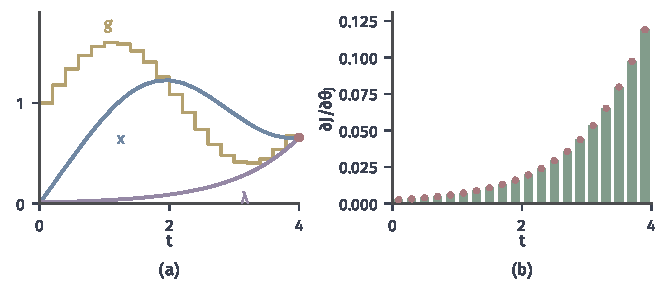
\includegraphics[width=112mm]{figures/06-differential-equations/01-ordinary-differential-equations/matplotlib/odesens-adjoint-gradient/figure.pdf}
  \caption{一次反向求解给出全部偏导数。方程$\dot{x}=-x+g$，$x_0=0$，$g$在$[0,4]$上分$20$段取常值（黄），$J=\tfrac12x(4)^2$。(a)状态$x$（蓝）与伴随$\lambda(t)=x(4)\mathrm{e}^{t-4}$（紫），红点是终端值。(b)绿色柱是伴随计算的$20$个偏导数，红点是逐分量中心差分。}
  \label{fig:odesens-adjoint-gradient}
\end{BookInlineFigure}

\paragraph{代价与失效情形}
表~\ref{tab:odesens-forward-adjoint}比较了前向与反向两种求导方式，其中$p$是参数个数，$k$是目标函数的个数。

\begin{BookInlineTable}
  \centering
  \caption{前向变分与反向伴随的代价对比。线性系统指沿同一条轨迹的$n$维线性初值问题。}
  \label{tab:odesens-forward-adjoint}
  \begin{tabular}{p{22mm}p{38mm}p{38mm}}
    \toprule
    & 前向变分 & 反向伴随 \\
    \midrule
    线性系统个数 & $p$个 & $k$个 \\
    是否保存轨迹 & 不需要，与状态同步 & 需要保存或重算 \\
    适合的情形 & 参数少、目标多 & 参数多、目标少 \\
    额外产出 & 完整的$\bm{P}(t)$ & 每一时刻的$\bm{\lambda}(t)$ \\
    \bottomrule
  \end{tabular}
\end{BookInlineTable}

伴随的主要代价是轨迹的存储。反向积分时要用到$\bm{A}(t)$，也就要用到$\bm{x}(t)$，长时间问题要在内存和重算之间权衡。$\bm{\lambda}$的大小也受放大因子控制：由式~\eqref{eq:odesens-adjoint-pullback}，
\[
 \lVert\bm{\lambda}(t)\rVert_2\leq\lVert\bm{\Phi}(T,t)\rVert_2\lVert\nabla\psi\rVert_2.
\]
敏感的问题里梯度本身就很大。

数值计算时还要注意，定理给的是连续问题的梯度。把伴随方程离散后算出的结果，一般不等于对离散格式求导的结果，两者只在步长趋于零时一致。定理的光滑性条件也不能省：右端在解经过的地方有$\lvert x\rvert$那样的折点时，$J$可能不可微。

得到梯度只是第一步，用它更新参数属于优化算法，可参考\BookChapterRef{chap:first-order-methods}{卷五第6章“一阶方法”}。当未知量是控制函数而不是有限维参数时，最优性条件需要更多工具，可参考\BookChapterRef{chap:continuous-time-optimal-control}{卷十第6章“连续时间最优控制”}。

\section{本章小结}
\label{sec:odesens-summary}

章首的问题是：把$x_0$改成$0.26$，或把增长率改$20\%$，$t=\ln3$时的值会差多少？现在有三种回答。Gronwall上界告诉我们，两种改变的影响分别不超过$0.01\,\mathrm{e}^{\ln3}=0.03$和$0.1$。变分方程给出一阶值$\tfrac43\times0.01=0.0133$与$0.0549$，后者与真实差$0.0547$很接近。若只需要一个目标对很多参数的梯度，伴随方程用一次反向求解就能得到。

四个工具输出的量不同，见表~\ref{tab:odesens-tools}。

\begin{BookInlineTable}
  \centering
  \caption{本章工具的对比。结论都针对给定解附近的紧时间段。}
  \label{tab:odesens-tools}
  \begin{tabular}{p{16mm}p{24mm}p{27mm}p{28mm}}
    \toprule
    工具 & 输出 & 主要条件 & 不能回答 \\
    \midrule
    Gronwall估计 & 曲线距离的上界 & 状态Lipschitz，系数可积 & 差的方向；长期趋势 \\
    变分方程 & 一阶响应$\bm{S}$、$\bm{P}$ & 对状态、参数$C^1$，导数有可积上界 & 大扰动；非光滑处 \\
    流映射 & 复合、逆、体积变化 & 解唯一，$C^1$ & 定义域外的解；长期轨道 \\
    伴随方程 & 目标函数的梯度 & 同变分方程，目标$C^1$ & 整个$\bm{P}(t)$；控制函数的最优性 \\
    \bottomrule
  \end{tabular}
\end{BookInlineTable}

几个相近的概念要分清。连续依赖只说解差随数据差趋于零；Lipschitz依赖给出速度，需要右端局部Lipschitz；可微依赖给出一阶系数，需要右端$C^1$，这三者一层比一层强，且不能由弱推强，$\dot{x}=-x\ln\lvert x\rvert$和$\dot{x}=\lvert x\rvert$分别是分界的反例。积分范数适合度量右端关于输入Lipschitz时的输入差，非线性增长时要限制输入的取值或改用更强的范数。残差和放大因子分别来自求解器和方程。

所有结论都是有限时间的。常数$\mathrm{e}^{\Lambda(T)}$可以很保守，也不说明长时间下解是靠拢还是分离，长期稳定需要卷九的额外结构和条件。第~\ref{chap:ode-numerical-methods}章的全局误差分析将回用本章的扰动估计，第~\ref{chap:transport-equations}章的输运方程回用流映射和体积变化。

